\documentclass{report}


\usepackage{amssymb}
\usepackage{amsthm}
\usepackage{latexsym}
\usepackage{amsmath}
\usepackage{verbatim}
%\usepackage{algorithm}
%\usepackage[noend]{algorithmic}
\usepackage{graphicx}
\usepackage{xcolor}
\usepackage{epsfig}
\usepackage{epstopdf}
%\usepackage[noend]{algorithmic}
%\usepackage{graphicx}
%\usepackage{xcolor}
\usepackage{epsfig}
\usepackage{multicol}
\usepackage{enumerate}
\usepackage{ulsy}
\usepackage[english]{babel}
\usepackage{media9}

%\newtheorem{complexConjugate}{Definition}
%\newtheorem{ZeeN}{Definition}
%\newtheorem{fourierTransform}{Definition}
%\newtheorem{convolution}{Definition}
%\newtheorem{spline}{Definition}
%\newtheorem{daubechies}{Theorem}

%
%\newtheorem{thm:ellCompleteness}{Theorem}
\newtheorem{thm:ellwave}{Theorem}
%%


\newtheorem{def:L2wavelet}[thm:ellwave]{Definition}
\newtheorem{def:multiresolutionanalysis}[thm:ellwave]{Definition}
\newtheorem{thm:Mallat}[thm:ellwave]{Theorem}

%
%\newtheorem{def:measurable}{Definition}
\newtheorem{MisSigmaAlgebra}[thm:ellwave]{Theorem}
%\newtheorem{def:measfunctions}{Definition}
%\newtheorem{thm:integ}{Theorem}
\newtheorem{thm:hilbert}[thm:ellwave]{Theorem}
\newtheorem{thm:vectorSpace}[thm:ellwave]{Lemma}
%\newtheorem{thm:innerProduct}{Lemma}
\newtheorem{thm:monoToneConv}[thm:ellwave]{Lemma}
\newtheorem{thm:metricCauchy}[thm:ellwave]{Theorem}

%\newtheorem{thm:identity}[thm:ellwave]{Theorem}

\newcommand{\N}{\mathbb{N}}
\newcommand{\Z}{\mathbb{Z}}
\newcommand{\R}{\mathbb{R}}
\newcommand{\C}{\mathbb{C}}
\newcommand{\M}{\mathbb{M}}
\newcommand{\ltoo}{\ensuremath{\ell^2 \left( \Z_{N} \right )}}
\newcommand{\F}{\mathcal{F}}
\newcommand{\pow}{\mathcal{P}}

\DeclareMathOperator{\range}{range}
\DeclareMathOperator{\closure}{\ensuremath{clos_d}}
\DeclareMathOperator{\error}{error}
\DeclareMathOperator{\spa}{span}
\title{Wavelets}

\author{Shane Scott \\ \small{Kansas State University Honors Program}}

\date{2012}


%{Department of Mathematics, Kansas State University, 138 Cardwell Hall, Manhattan, KS 66506-2602,USA1}

\begin{document}

%\begin{titlepage}
%\begin{center}
%\textsc{}
%\end{center}
%\end{titlepage}
\maketitle

\begin{abstract}
Fourier spectral analysis provides methods of signal compression and approximation, but presents some limitations to practical implementations. The Fourier transform of a signal may be thought of as its representation over a (pseudo) basis of complex exponentials, which while localized in frequency space, are delocalized in time. In contrast with the Fourier basis, a wavelet basis can be both frequency and time localized. Such a basis allows transformations between representations to be calculated locally, and partial representations can often be calculated even when only a portion of the signal is known.   We demonstrate and compare low-loss signal compression using both methods. Through a discussion of the advantages of wavelet representations we will motivate a theoretical discussion of alternative bases and give proofs of their construction and in the space of square summable complex sequences and the space of square Lebesgue integrable functions.
\end{abstract}

\pagenumbering{roman}
\tableofcontents
\listoffigures


\section*{Acknowledgement}

This work was supported by a scholarship from the Center for the Integration of Undergraduate, Graduate, and Postdoctoral Research of the Mathematics Department at Kansas State University under the direction of Dr. Virginia Naibo and in collaboration with Brian Moore and Vincent Pigno.

\begin{center}
\begin{figure}[!hf]
\center
\includegraphics[height=1.1cm]{icenterlogo2}
\end{figure}
\end{center}
\section*{Notation}
%\begin{multicols}{2}
\begin{small}
\begin{table}[!hf] \small
\begin{tabular}{ l c l}
$\Z$ && the set of integers\\
$\Z^+$ &&  the set of positive integers\\
 $\N$ &&  the set of non-negative integers\\
$\R$ &&  the set of real numbers\\
 $\R^+$ &&  the set of positive real numbers\\
  $\R^+_0$ &&  the set of non-negative real numbers\\
$\C$ &&  the set of complex numbers\\
$\pow (A)$&& set of all subsets of $A$\\ 
$A^c$&& set compliment of $A$\\ 
$\ell^1 (\Z)$ &&  the absolutely of summable sequences\\
$\ell^2 (\Z)$ &&  the set of square summable sequences\\
$\ell^2 (\Z_N)$ &&  $N$ length complex vectors\\
$L^2 (A )$ &&  the set of square integrable complex valued functions on $A$\\
$\closure A$ && $d$ induced metric topology closure of $A$\\
$\sum_{a\in A} z(a) $ &&  the summation of $z$ over set $A$\\
$\prod_{a\in A} z(a) $ &&  the product of $z$ over set $A$\\
$\int_A f(x) dx$ &&  the Lebesgue integral of $f$ over $A$\\
$\langle v|w \rangle$ &&  inner product of $v$ and $w$\\
 $ v\ast w$  && convolution of $v$ and $w$\\
$v \perp w$&& $v$ orthogonal to $w$\\
$V \oplus W$&& orthogonal direct sum of $V$ and $W$\\
$|z|$&& modulus of $z$ \\
$\|z\|$&& norm of $z$ \\
$\overline z$&& complex conjugate of z\\
$\tilde z$&& conjugate reflection of z\\
 $R_nz$ && $n^{th}$ translation of $z$\\
$\hat z$&&Fourier or Discrete Fourier transform of z\\
 $\check f$ && inverse Fourier transform of $f$\\
$f:A \to B$&& $f$ is a set function from $A$ to $B$\\
$f:a \mapsto b$&& $f$ maps $a$ to $b$\\
$\delta$ && Dirac delta sequence \\
$I_n$&& $n \times n$ identity matrix\\
\end{tabular}
\end{table}
\end{small}

%\end{multicols}

\pagenumbering{arabic}

\chapter{Introduction: Wavelet Compression of a Digital Signal}
\label{ch:intro}

Informally wavelets are vectors in a space whose translations and dilations span the space. Often wavelets may be chosen which are localized in both their temporal and frequency representations. Wavelets are of interest both to theory and application, so it may be best to demonstrate by an example. The following informal presentation of wavelet applications to data compression techniques may help to motivate the theoretical discussion of their existence and construction that follows.

In an increasingly data-filled age where few are unfamiliar with concepts of streaming or data transfer, more and more are routinely initiated merely from internet exposure, even while the underlying mathematics goes unrecognized. Efficiency of such data transmission is of great concern with the current proliferation of sites streaming music, video, photos.   Signals (such as electrical and optical signals speeding through cables and antennas across the country) are best modeled as vectors in the space:
$$
L^2 (\R )=\left \{ v: \R \to \C \  \middle | \ \int_\R |v(t)|^2 dt <\infty \right \}.
$$
In the digital landscape, the discrete versions of signals instead lie in 
$$
\ell^2 (\Z) = \left \{ v: \Z \to \C  \middle | \ \sum_{n\in \Z} |v(n)|^2 <\infty \right \},
$$
or in the practice of computation, we may have discrete, finite length vectors
$$
\ell^2 (\Z_N) = \left \{ v: \Z_N \to \C \right \}.
$$
These are simply $N$ length vectors of complex values. We will develop some of the theory of wavelets in these spaces. But for now, let's consider the signal $z \in \ell^2 (\Z_N)$ shown in Figure \ref{fig:wak}.

\begin{figure}
\center
\caption{A Walken Signal $z$}
\label{fig:wak}
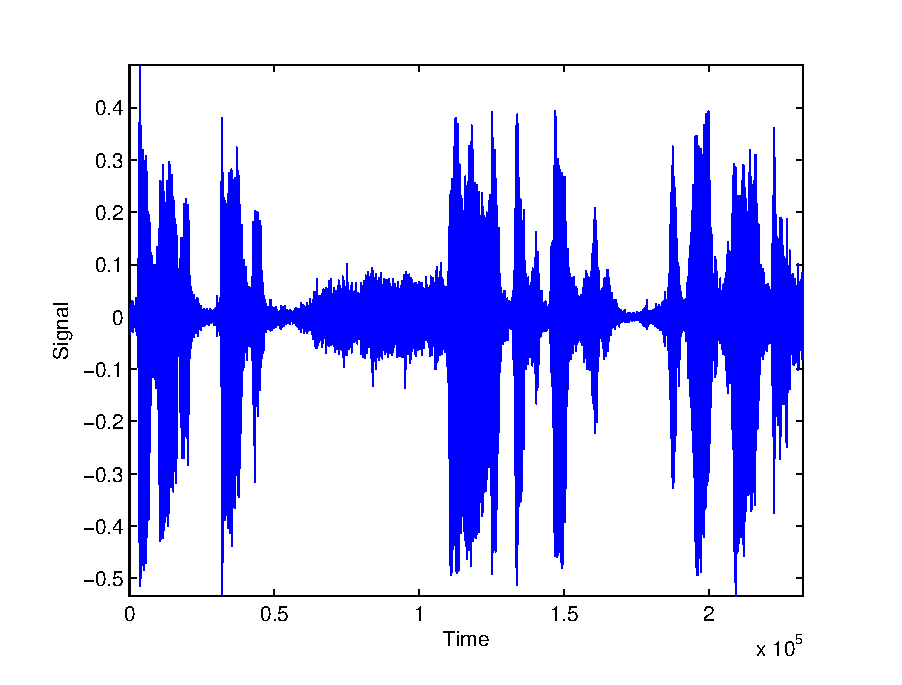
\includegraphics[height=8cm]{figure1.eps}

\includemedia[
  addresource=igottafever.mp3,
  flashvars={
    source=igottafever.mp3
&autoPlay=true
  }
]{\fbox{Play}}{APlayer.swf}
\end{figure}

The signal $z$ represents a digital sound signal of Christopher Walken performing a line from an April 8, 2000, \emph{Saturday Night Live} sketch. (Press the play button in Figure \ref{fig:wak} to listen to the clip.) Suppose we are faced with the problem of storing a great many such signals in a database, or transmitting the signal as fast as possible. Lossy compression techniques to such problems look to find ways of representing signals (or at least an approximation) with as little information as possible. A fairly simple method of digital compression is Fourier compression.

The discrete fourier transform of $z$ is $\hat z$, also an $N$ length vector, given by the formula
\begin{equation}
\label{equation:Fourier}
\hat z (m) = \frac{1}{\sqrt{N}}\sum^{N-1}_{n=0} z(n) e^{-2\pi i m n/N}.
\end{equation}
This transformation is reversed by the inverse transformation
\begin{equation}
\label{equation:Finverse}
z (n) = \frac{1}{\sqrt{N}}\sum^{N-1}_{m=0} \hat z(m) e^{2\pi i m n/N}=\left \langle \frac{e^{-i2\pi mn/N}}{\sqrt N} \middle | \hat z \right \rangle,
\end{equation}
and we can then think of $\hat z$ as the representation of $z$ over a basis of complex exponentials (essentially sine waves):
$$
z(n)= \sum^{N-1}_{m=0} \left \langle \frac{e^{i2\pi mn/N}}{\sqrt N} \middle | z \right \rangle \frac{e^{i2\pi mn/N}}{\sqrt N},
$$
while $z$ is its own representation over the standard basis. In this sense $z$ is the \emph{temporal} or \emph{spatial} representation while $\hat z$ is the \emph{frequency} space representation of $z$. The component-wise absolute value of $\hat z$ is called the \emph{spectrum} of $z$. The spectrum of Mr. Walken's line is shown in Figure \ref{fig:Fwak}. 

\begin{figure}
\center
\caption{The Walken Spectrum $|\hat z|$}
\label{fig:Fwak}
\includegraphics[height=8cm]{Fourier.eps}
\end{figure}

Notice that a small number of positions of $\hat z$ have a large value, while many have values close to zero. Thus we can discard many of these position and replace them only with zero, we can perform the inverse Fourier transform to obtain a very close approximation of $z$. By transmitting only the positions of $\hat z$ above some threshold value, we have much less data to transmit, but can still reconstruct a very close approximation to $z$. The Fourier compression algorithm at this point goes as follows. To compress and send a $p$ percent sized representation of $z$:
\begin{enumerate}
\item Calculate $\hat z$.
\item Order the values of $\hat z$ by their values in modulus and calculate $a$, their $p^{th}$ percentile.
\item If a component of $\hat z$ is less that $a$ in absolute value, discard it and replace it with $0$.
\item Transmit the positions and values of the non-zero positions of $\hat z$.
\item Reconstruct the approximation by taking the inverse Fourier transform.
\end{enumerate}

\begin{figure}
\center
\caption{The 90\% Compressed Walken Spectrum $|\hat z|$}
\label{fig:90Fwak}
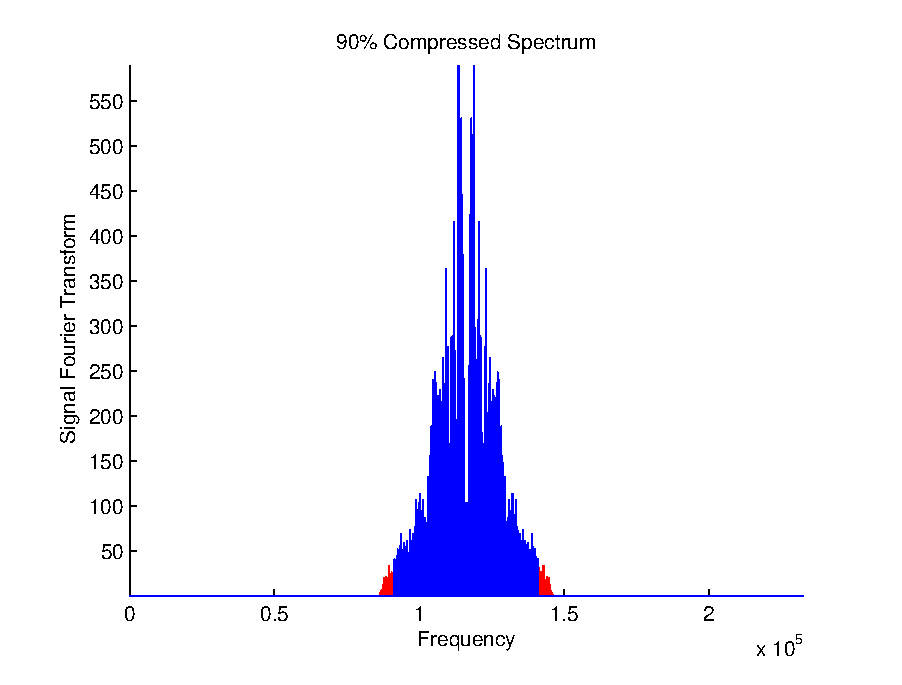
\includegraphics[height=7cm]{90four.eps}


\end{figure}

\begin{figure}
\center
\caption{The 90\% Compressed Walken Signal $z$}
\label{fig:I90Fwak}
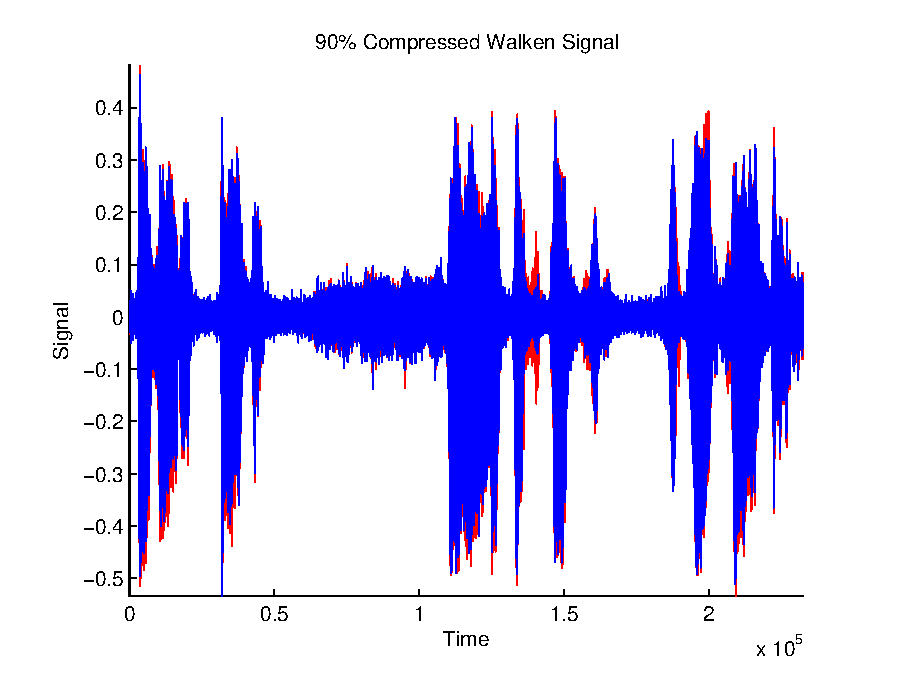
\includegraphics[height=7cm]{90fourRec.eps}

\includemedia[
  addresource=90Fourier.mp3,
  flashvars={
    source=90Fourier.mp3
&autoPlay=true
  }
]{\fbox{Play}}{APlayer.swf}
\end{figure}

\begin{figure}
\center
\caption{The 95\% Compressed Walken Spectrum $|\hat z|$}
\label{fig:95Fwak}
\includegraphics[height=7cm]{95four.eps}
\end{figure}

\begin{figure}
\center
\caption{The 95\% Compressed Walken Signal $z$}
\label{fig:I95Fwak}
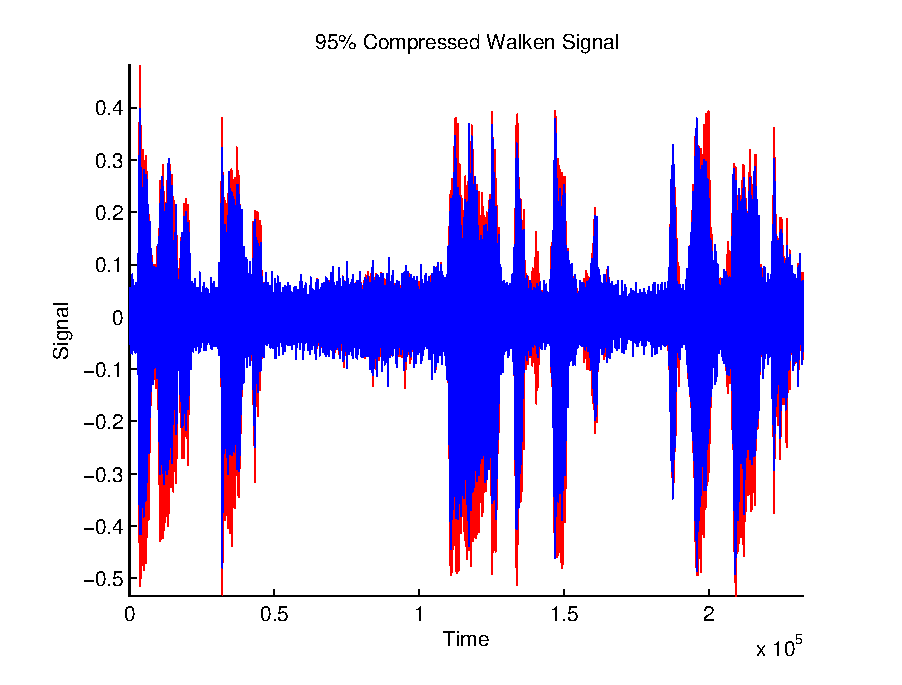
\includegraphics[height=7cm]{95fourRec.eps}

\includemedia[
  addresource=95Fourier.mp3,
  flashvars={
    source=95Fourier.mp3
&autoPlay=true
  }]{\fbox{Play}}{APlayer.swf}
\end{figure}

Figures \ref{fig:90Fwak} and \ref{fig:95Fwak} show the $90\%$ and $95\%$ compressed spectrum of $z$ in blue while the original is shown for comparison in red. (The thickness of the graph lines in the figures obscures the sparsity of the non-zero coefficients post-compression, but only 10\%/5\% remain.) Figures \ref{fig:I90Fwak} and \ref{fig:I95Fwak} show the reconstructed approximation to $z$ in blue with the original $z$ in red. Press the "Play" button by their graph to listen. Thus we can reduce by $95\%$ or more the amount of data describing  $z$ and still have a very close approximation to Mr. Walken's line.

This technique is good, but still has a number of drawbacks. Note first that in the compressed versions of $z$ as we increase the compression ratio the signal to background ratio is getting much worse, that is most of the information loss occurs on the most important parts of the signal. But for modern applications like web streaming, this method has an even bigger problem. Note that the inversion formula for $z$ from $\hat z$ ( Eq. \ref{equation:Finverse}) each component of $z$ must be calculated using every component of $\hat z$, so the inversion calculation cannot begin until all of $\hat z$ is transmitted, which is decidedly not how web streaming operates. We call this problem the time \emph{delocalization} of the complex exponential basis. Without going into detail, we can say compression of video signals works much the same way. Take a peak at this video clip of Mr. Walken delivering his line (Figure \ref{fig:wakclip}).

\begin{figure}[!hb]
\center
\caption{Christopher Walken on SNL}
\label{fig:wakclip}
\includemedia[
	deactivate=pageclose,
	width=200pt, height=90pt,
	addresource=walkenclip.mp4,
	flashvars={src=walkenclip.mp4 & loop=false &autoPlay=true}
]{\fbox{Play}}{StrobeMediaPlayback.swf}
\end{figure}

Although this example of Mr. Walken is a two dimensional example, the two dimensional case is very similar to that of the one dimensional; a Fourier transform exists and the coefficients depend on every spatial pixel, that is, they are not spatially localized. Observe that the background behind Mr. Walken changes very little throughout the clip. A better algorithm might avoid sending redundant information to update the background, but because the values of $\hat z$ depend on all components of $z$, (see Eq. \ref{equation:Fourier}), we cannot avoid sending some of this information.  That is, the standard basis which expresses the time representation $z$ is delocalized in the frequency space. But a modification of the compression algorithm can overcome these drawbacks.

The compression algorithm we have expressed depends only on having a basis over which the representation of $z$ has as many zeros or small values, so instead we can hope to find a  basis which is localized both in the standard space and in the frequency space. Qualitatively this means that we will find a basis of vectors which have only a small section of non-zero components and whose Fourier transforms have only a small section of non-zero coefficients. One example is the Mexican Hat wavelet, whose time and frequency representations are shown in Figures \ref{fig:Mhat} and \ref{fig:fMhat}.  A basis may be formed via their spatial translations, which will avoid the localization objection raised to the complex exponential basis. A detailed technical discussion of this may be found in the succeeding chapters.

\begin{figure}
\center
\caption{The Mexican Hat wavelet in standard space}
\label{fig:Mhat}
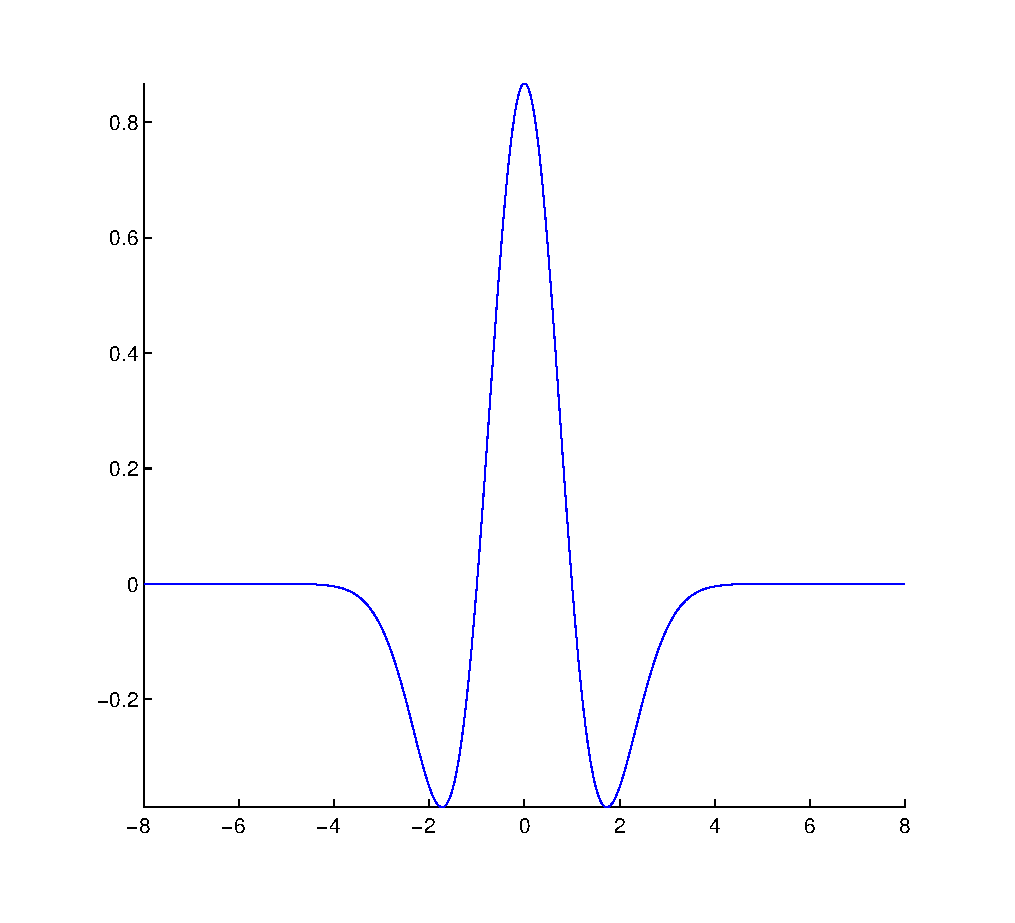
\includegraphics[height=5.25cm]{mexhat.eps}

\caption{The Mexican Hat wavelet in frequency space}
\label{fig:fMhat}
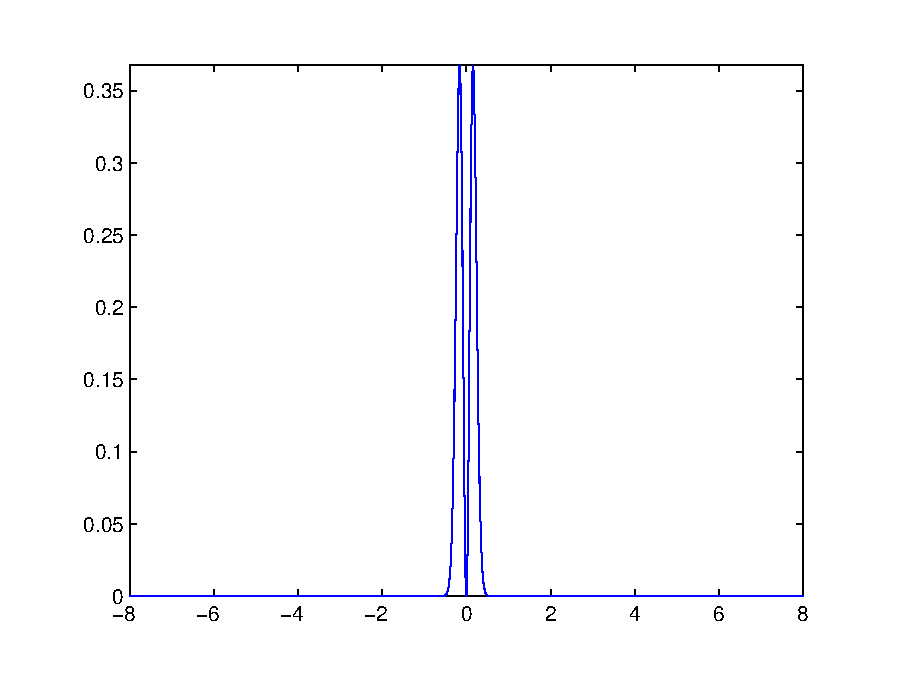
\includegraphics[height=5.25cm]{mexhatFour.eps}
\end{figure}

For discrete finite length vectors we form a first stage wavelet basis by taking the even spatial translations of two vectors $u$ and $v$. We will choose $u$ such that only low frequency components are non-zero, while $v$ will have high frequency components non-zero. Figure \ref{fig:d4} shows one such example, Daubechies's D4 wavelet filter pair.

\begin{figure}
\center
\caption{The D4 wavelet in space}
\label{fig:d4}
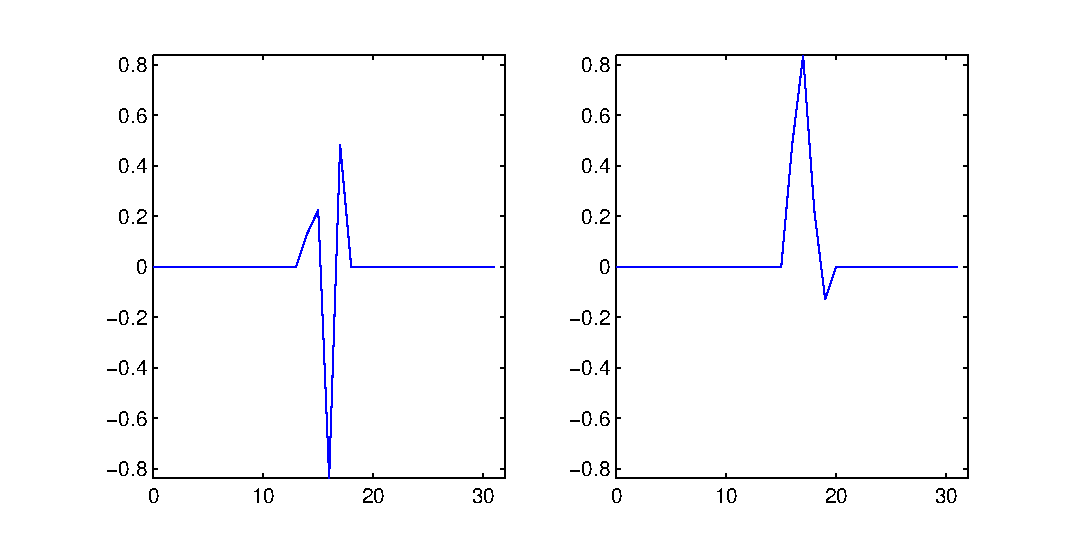
\includegraphics[height=5.25cm]{d4}

{(Left) High frequency filter. (Right) Low frequency filter.}

\caption{The D4 wavelet in frequency space}
\label{fig:Fd4}
\includegraphics[height=5.25cm]{d4Four}

{(Left) High frequency filter spectrum. (Right) Low frequency filter spectrum.}
\end{figure}

Then the components of $z$ represented over the translations of $u$ will contain an $N/2$ length approximation of $z$, while the components of $z$ represented over the translations of $v$ will contain the details of $z$. Figure \ref{fig:stage1} shows the  representation of $z$ in the wavelet basis. The first half is an approximation of $z$, while the second contains the details needed to reconstruct $z$. We can the revise the compression algorithm to discard the detail components of the wavelet representation of $z$. This will (most of the time) maintain the original signal to noise ratio of $z$, the first objection we raised to the Fourier compression algorithm. But by discarding only details, we are limited to 50\% compression. By decomposing the N/2 wavelet approximation over an $N/2$ length wavelet basis, and iterating this process, we can continue to produce more detail components which can be discarded to compress the signal. Our new algorithm to compress $z$ by $p$ percent and transmit is as follows.




Let $\ell$ be the minimal integer satisfying $p \leq 1-2^{-\ell}$ and assume $N$, the length of $z$, satisfies $2^\ell | N$. Let $z_{(0)}=z$. Let $p'=\frac{p}{1-2^{-\ell}}$.
\begin{enumerate}
\item While $1 \leq k \leq \ell$
	\begin{enumerate}[a.]
	\item Form $z_{(k)}$ from $z_{(k-1)}$ by replacing the length low frequency approximation of $z_{(k-1)}$  (the first $2^{-k}N$ components) by its representation over an $2^{-k}N$ length first stage wavelet basis.
	\end{enumerate}
\item Order the detail components of $z_{(\ell)}$ (the last  $N(1-2^{-\ell})^{-1}$ components) by their moduli and calculate $a$, their $p'^{th}$ percentile.
\item If a detail component of $z_{(\ell)}$ is less than $a$ in modulus, discard it and replace it with $0$.
\item Transmit the positions and values of the non-zero positions of $z_{(\ell)}$.
\item Reconstruct the $N$ length approximation of $z$ by taking the inverse wavelet transformations.
\end{enumerate}
(In fact, a $\ell^{th}$ stage wavelet basis can be calculated directly so that the calculation of $z_{(\ell)}$ need not be performed iteratively.) Because this new algorithm retains the low frequency approximation coefficients,  it retains a signal to noise ratio in the compressed signal better than the Fourier algorithm. The localization of the wavelet basis means we may begin reconstruction while only a few components have been transmitted. Figures \ref{fig:stage1} through \ref{fig:stage4p95} show the iterative calculation of $z_{(\ell)}$ using Daubechies's D4 wavelet, a 90\% and 95\% compression, and their reconstructed approximations of $z$. Again the compressed signals are shown in blue over the original in red. Listen to the signal by pressing the play button  and compare it with the Fourier method. While the same amount of compression is achieved with both, the wavelet compressed signal has discarded much of the background noise, while the Fourier method sounds like it has amplified it. Figure \ref{fig:err} shows a comparison of the 
error\footnote {
%\mbox{
The percent error for a compressed $z'$ from signal $z$ is given by $\error(z',z)=\frac{\|z'-z\|}{\|z\|}$ where $\|\cdot\|$ is the vector space norm. See the later discussion.
%}
}
between the Fourier and wavelet compression techniques. Observe that in this example, the Fourier method has better error values for lower levels of compression, although for compression over 80\%, the wavelet method produces lower error. Compressing with a higher stage basis also appears to continue to improve the error of the compression. Bear in mind that because the wavelet compression method discards more noise information, a portion of its error is irrelevant to our purpose, and in some contexts even a desirable denoising. Then a wavelet compression approach out-performs the Fourier compression in terms of  high-compression error, localization, and signal-to-noise constancy.

The iterative levels that are naturally constructed by wavelet bases lend themselves to many other applications. Because the compression separates a rough approximation and detail information, it enables algorithms which examine first rough approximations of signals then further examine the details of signals if something of interest is revealed, as might be of interest to remote sensing or image recognition applications.
Many uses of wavelets are found in the literature. In the discussion that follows we will look instead towards the theory surrounding their existence and construction.


\begin{figure}[!hb]
\center
\caption{1st Stage Wavelet Representation $z_{(1)}$}
\label{fig:stage1}
\includegraphics[height=5.25cm]{stage1}

\caption{2st Stage Wavelet Representation $z_{(2)}$}
\label{fig:stage2}
\includegraphics[height=5.25cm]{stage2}
\end{figure}

\begin{figure}
\center
\caption{3rd Stage Wavelet Representation $z_{(3)}$}
\label{fig:stage3}
\includegraphics[height=5.25cm]{stage3}

\caption{4th Stage Wavelet Representation $z_{(4)}$}
\label{fig:stage4}
\includegraphics[height=5.25cm]{stage4}

\caption{90\% Compressed 4th Stage Wavelet Representation $z_{(4)}$}
\includegraphics[height=5.25cm]{stage4p9}
\label{fig:stage4p9}
\end{figure}

\begin{figure}
\center
\caption{90\% Wavelet Compressed $z$}
\label{fig:stage4p9}
\includegraphics[height=5.25cm]{reConstructp9}

\includemedia[
  addresource=90D4.mp3,
  flashvars={
    source=90D4.mp3
&autoPlay=true
  }]{\fbox{Play}}{APlayer.swf}

\caption{95\% Compressed 5th Stage Wavelet Representation $z_{(5)}$}
\label{fig:stage4p95}
\includegraphics[height=5.25cm]{stage4p95}

\caption{95\% Compressed $z_{(5)}$}
\label{fig:stage4p95}
\includegraphics[height=5.25cm]{reConstructp95}

\includemedia[
  addresource=95D4.mp3,
  flashvars={
    source=95D4.mp3
&autoPlay=true
  }]{\fbox{Play}}{APlayer.swf}
\end{figure}

\begin{figure}
	\center
	\caption{Comparison \% Error by Compression Ratio}
	\label{fig:err}
	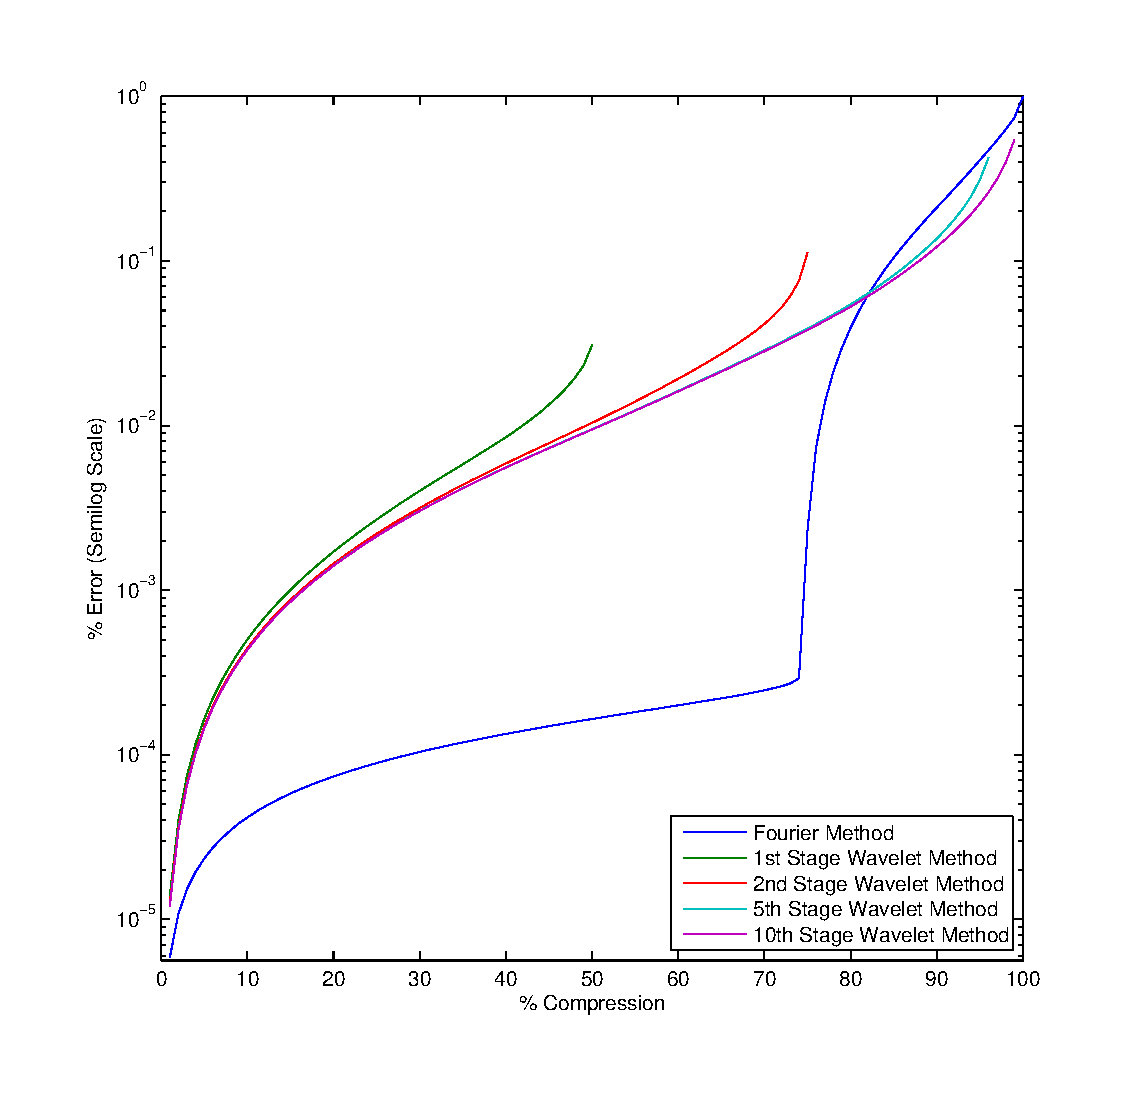
\includegraphics[width=12cm]{errorsPlot}
\end{figure}


\chapter{Discrete Wavelets}
\label{ch:techintro}

Wavelets over the spaces $\ell^2 (\Z)$ and $\ell^2 (\Z_N)$ are widely used in application, and we shall build our theory of continuous wavelets off the discrete foundation.   We begin by defining our notation.

 For a set $A$, we write its power set as $\pow (A)=\{ U \ | \ U \subseteq A \}$ .We will write $\Z$ to refer the integers, and $\R$ to refer to the the field of real numbers. $\Z^+$ and $\R^+$ will refer to the positive integers and real numbers, respectively. We write $\C$ for the field of complex numbers. For a complex number $z= x + iy$ with $x,y \in \R$ and $i =\sqrt{-1}$ we write the {complex conjugate} of $z$ as $\bar z = x - iy$.

%%%%%%%
\begin{comment}
\begin{ZeeN}
We will consider a length $N$ vector as a map $v: \{0,\ldots, N-1\} \to \C$. We refer to the set of all such vectors as $\Z_N$. The vector space $\ltoo$ is the set of vectors $\Z_N$ equipped with the scalar field $\C$ and the inner product $\langle \cdot | \cdot \rangle: \ltoo \times \ltoo \to \C$ where for $v,w \in \ltoo$
$$
\langle v | w \rangle= \sum^{N-1}_{n=0} \overline{v(n)}{w(n)}
$$
and the $\ltoo$ norm
$$
\|v \|=\langle v | v \rangle ^{\frac{1}{2}} = \left ({\sum^{N-1}_{n=0} |v(n)|^2}\right ) ^\frac{1}{2}.
$$
\end{ZeeN}

\begin{fourierTransform}
We define the \emph{discrete Fourier transform} as the map $\F: \ltoo \to \ltoo$ such that 
$$
\F (v) (m) = \sum^{N-1}_{n=0} v(n) e^{-2\pi i m n/N}.
$$
We will typically write the discrete Fourier transform of $v$ as $\hat v = \F (v)$
\end{fourierTransform}

For $N$ length vectors it is easy to consider the vector as its periodic extension, that is we will write
$v(n+kN)=v(n)$ for $n \in \{0,\ldots,N-1\}$ and any $k \in \Z$.


We define the \emph{convolution} of vectors in $\ltoo$ as the binary operation $( \cdot \ast \cdot ): \ltoo \times \ltoo \to \ltoo$ where for $v,w \in \ltoo$ we have
$$
(v \ast w) (m)= \sum^{N-1}_{m=0} v(n-m)w(m)
$$
\begin{align}
v \ast \tilde w (n) &=  \sum_{m=0}^{N-1} v(n-m)\tilde w (m) \\
&=  \sum_{m=0}^{N-1} v(m)\tilde w (n-m) \\
&=  \sum_{m=0}^{N-1} v(m)\tilde w (m-n) \\.
\end{align}
\end{comment}
%%%%%%%%%%%


An infinite, discrete signal is usually thought of as a vector in 
$$
\ell^2 (\Z)=\left \{ v: \Z \to \C \ \middle | \ \sum_{n\in \Z} |v(n)|^2 < \infty \right \}.
$$
Most of the concepts needed for a discussion of wavelets in $\ell^2 (\Z)$ are directly analogous to those of $\ltoo$, the space of length $N$ complex vectors, though the situation is slightly complicated by concerns of convergence. We will discuss the infinite case, and note that the finite length case is analogous, though without the necessity of limits. It is straightforward to check that $\ell^2 (\Z)$ is a vector space under the obvious point-wise addition and scalar multiplication. We are able to equip $\ell^2 (\Z)$ with the inner product
$$
\langle v | w \rangle = \sum_{n \in \Z} \overline{v(n)}w(n),
$$
and the norm
$$
\|v\|=\langle v | v \rangle^\frac{1}{2}
$$
which provides us with the metric $d(v,w)=\|v-w\|$. We will state without proof that $\ell^2 (\Z)$ is in fact Cauchy complete with respect to this metric, making it a complete inner product space or Hilbert space (see the appendix for more information).

 We distinguish one particular sequence called the \emph{Dirac delta} $\delta \in \ell^2 (\Z)$ where $\delta(n)=1$ if $n=0$ and $\delta(n)=0$ if $n \neq 0$.
We call $\ell^1 (\Z)$ the space defined by
$$
\ell^1(\Z)=\left \{ v: \Z \to \C \ \middle | \ \sum_{n\in \Z} |v(n)| < \infty \right \}
$$
for which we note $\ell^1 (\Z) \subset \ell^2 (\Z)$. To see this consider $v \in \ell^1 (\Z)$. It must be that $\lim_{n\to -\infty} v(n)=0$ and $\lim_{n\to \infty} v(n)=0$. Then there is some $N \in \Z^+$ such that $n \geq N$ implies $|v(n)|<1$. Then if $n>N$
\begin{align*}
\sum_{k=-n}^{n}|v(k)|^2 &=\sum_{k=-N}^{N}|v(k)|^2+\sum_{N<|k|\leq n}|v(k)|^2 \\
&\leq \sum_{k=-N}^{N}|v(k)|^2+\sum_{N<|k|\leq n}|v(k)|\\
&\leq \sum_{k=-N}^{N}|v(k)|^2+\sum_{k \in \Z}|v(k)|\\.
\end{align*}
So we see the the sequence of partial sums $\sum_{k=-n}^{n}|v(k)|^2$ is real, monotone, and bounded, so must converge to some finite number. Hence $v \in \ell^2 (\Z)$. The reverse inclusion is of course false. Take, for example, the sequence $z: \Z \to \C$ with $z(n)=(1/n)$ for $n\neq 0$ and $z(0)=0$. We know that$\sum_{n \in \Z} \frac{1}{n}$ diverges so naturally $\sum_{k\in \Z} |z(k)|$ also diverges, while $\sum_{n \in \Z} |z(n)|^2$ converges to $\frac{\pi^2}{2}$.

A number of operations on $\ell^2 (\Z)$ will be useful in studying and constructing wavelets.
The \emph{conjugate reflection} map  $\tilde {\cdot}: \ell^2 (\Z) \to \ell^2 (\Z)$ takes $v$ to $\tilde v$ defined by
$$
\tilde v (n) = \overline{v(-n)}.
$$
The \emph{translations maps} $R_k: \ell^2 (\Z) \to \ell^2 (\Z)$ are defined by
$$
R_kv(n)=v(n-k)
$$
where $k \in \Z$. We call $u \in \ell^2(\Z)$ \emph{even translate orthonormal} if the set
$$
\{R_{2k}u \ | \ k \in \Z\}
$$
is orthonormal. For such a vector we will call its \emph{sister wavelet} the sequence $v$ defined by
$$
v(k)=(-1)^{k-1}\overline{u(1-k)}.
$$
The even translate orthonormality of $v$ is equivalent to that of $u$. Observe that the sister of the sister of $u$ is $u$ itself and
\begin{align*}
\langle v | R_{2m} v \rangle &= \sum_{k \in \Z}\overline{v(k)}{v(k-2m)}\\
 &= \sum_{k \in \Z}(-1)^{k-1}{u(1-k)}(-1)^{k-2m-1}\overline{u(1-k+2m)}\\
  &= \sum_{k \in \Z}\overline{u(1-k+2m)}{u(1-k)}\\
    &= \sum_{k \in \Z}\overline{u(k)}{u(k-2m)}\\
    &= \langle u | R_{2m} u \rangle\\.
\end{align*}
We call a basis $B$ of $\ell^2 (\Z)$ a \emph{first-stage wavelet basis} if there is some $u \in B$ such that $u$ is even translate orthonormal with sister wavelet $v$ and
$$B=\{R_{2k}u \ | \ k \in \Z \}\cup\{R_{2k}v \ | \ k \in \Z \}.$$
We write $L^2 [-\pi,\pi)$ for the space of square integrable functions on  $[-\pi,\pi)$:
$$
L^2 [-\pi,\pi)=\left\{ f: [-\pi,\pi) \to \C \ \middle | \ \int_{-\pi}^\pi |f(t)|^2  \ dt\right\}.
$$ 
We define the Fourier transform on $\ell^2 (\Z)$ as the map $\F: \ell^2 (\Z) \to L^2 [-\pi,\pi) $ such that $\F(z)=\hat z$ defined by
$$
\hat z (\omega) = \frac 1 {\sqrt {2\pi}} \sum_{n \in \Z} z(n)e^{in\omega}.
$$
It can be shown that the Fourier transform has inverse $\F^{-1}: L^2[-\pi,\pi) \to \ell^2(\Z)$ where  $\F^{-1}: f \mapsto \check{f}$ such that
 $$
 \check f (n) = \frac 1 {\sqrt{2 \pi}} \int_{-\pi}^{\pi} f(\omega)e^{-in\omega} \ d\omega,
 $$
and we have $\check{\hat{z}}=z$ and $\hat{\check{f}} =f$. If we consider that $L^2 [-\pi,\pi)$ itself is a Hilbert space (see appendix) equipped with its own inner product 
$$
\langle f | g \rangle=\int_{-\pi}^{\pi} \overline{f}(\omega)g(\omega) \ d\omega,
$$
then we can write $\hat z (\omega) =\left \langle \frac{e^{-in\omega}}{\sqrt{2\pi}} \middle |z \right \rangle$ where the inner product is in $\ell^2 (\Z)$ and $\check f (n) =\langle \frac{e^{in\omega}}{\sqrt{2\pi}}|f \rangle$ where the inner product is that of $L^2 [-\pi,\pi)$. The symmetry between the inner products of these two spaces is even greater, and given by Parseval's formula:
$$
\langle z|w \rangle=\langle \hat z | \hat w \rangle
$$
where again the first inner product is over $\ell^2 (\Z)$ while the second is that of $L^2 [-\pi,\pi)$. We note a few helpful Fourier relations:
\begin{align*}
\sqrt{2\pi}\hat \delta (\omega)&= \sum_{n\in \Z}\delta(n) e^{in\omega}=1\\ ,
\end{align*}
\begin{align*}
\widehat{(-1)^n z(n)}(\omega)&= \sum_{n\in \Z}(-1)^n z(n) \frac{e^{in\omega}}{\sqrt{2 \pi}}\\
&= \sum_{n\in \Z}z(n) \frac{e^{in(\omega+\pi)}}{\sqrt{2\pi}}\\
&= \hat z {(\omega+\pi)},
\end{align*}
\begin{align*}
\widehat{R_k z}(\omega)&= \sum_{n\in \Z}z(n-k) \frac{e^{in\omega}}{\sqrt{2\pi}}\\
&= \sum_{n\in \Z}z(n) \frac{e^{in\omega}}{\sqrt{2\pi}}e^{ik\omega}\\
&= \hat z {(\omega)}e^{ik\omega}.
\end{align*}


The operation of \emph{convolution} is a binary operation  $\cdot \ast \cdot : \ell^1(\Z) \times \ell^1(\Z) \to \ell^2 (\Z)$ where
\begin{align*}
z \ast w (n) & =\sum_{m \in \Z} z(n-m)w(m)\\
& =\sum_{m \in \Z} R_n \tilde z(m)w(m)\\
& =\langle R_n \tilde z| w \rangle \\.
\end{align*}
The convolution has the useful property that $\widehat{z \ast w}=\sqrt{2\pi}\hat z \hat w$. 

\begin{thm:ellwave}
\label{thm:ellwave}
Let $u \in \ell^1 (\Z)$ be even translate orthonormal. Then if we define the sister wavelet $v$ by
$$
v(k)=(-1)^{k-1}\overline{u(1-k)}.
$$
Then $B=\{R_{2k}u \ | \ k \in \Z \}\cup\{R_{2k}v \ | \ k \in \Z \}$ is an orthonormal basis for $\ell^2 (\Z)$, and we call $B$ a first stage wavelet basis.
\end{thm:ellwave}

\begin{proof}
Observe that if $u$ is even translate orthonormal, then $\langle R_{2m}u |  u \rangle = \delta(m)$ and we have by Parseval's formula that
\begin{align*}
\langle u |  R_{2m}u \rangle &= \left \langle \hat u \middle |  \widehat{R_{2m}u}  \right \rangle\\
&= \int_{-\pi}^{\pi}\overline {\hat u}(\omega) \hat u(\omega) e^{-i2m\omega} d\omega\\
&= \int_{-\pi}^{0} |\hat u(\omega)|^2 e^{-i2m\omega} d\omega+\int_{0}^{\pi} |\hat u(\omega)|^2 e^{-i2m\omega} d\omega\\
&= \int_{0}^{\pi} |\hat u(\omega+\pi)|^2 e^{-i2m\omega} d\omega+\int_{0}^{\pi} |\hat u(\omega)|^2 e^{-i2m\omega} d\omega\\
&= \int_{0}^{\pi}  \left(|\hat u(\omega)|^2+|\hat u(\omega+\pi)|^2 \right) e^{-i2m\omega} d\omega
\end{align*}
Then
\begin{align*}
\delta(m)&= \int_{-\pi}^{\pi}  \frac{1}{2}\left(\left|\hat u\left(\frac{\omega}{2}\right)\right|^2+\left|\hat u\left(\frac{\omega}{2}+\pi\right)\right|^2 \right) e^{-im\omega} d\omega.
 \end{align*}
 By taking the Fourier transform on both sides we have for $\omega \in [-\pi,\pi)$
 $$
\frac 1 {\sqrt{2\pi}}=\frac{1}{2}\left|\hat u\left(\frac{\omega}{2}\right)\right|^2+\frac{1}{2}\left|\hat u\left(\frac{\omega}{2}+\pi\right)\right|^2,
 $$
or for $\omega \in [0,\pi)$
\begin{equation}
\label{eq:a}
\frac 2 {\sqrt{2\pi}}=\left|\hat u\left(\omega \right)\right|^2+\left|\hat u\left(\omega+\pi \right)\right|^2.
\end{equation}
The same argument applied to $v$ yields that
\begin{equation}
\label{eq:b}
\frac 2  {\sqrt{2\pi}}=\left|\hat v\left(\omega \right)\right|^2+\left|\hat v\left(\omega+\pi \right)\right|^2
\end{equation}
is equivalent with $v$ being even translate orthonormall.
Consider the Fourier transform of $v$ calculated by its definition through $u$
\begin{align*}
\hat v (\omega) &= \sum_{k\in \Z} (-1)^{k-1}\overline{u(1-k)} \frac{e^{ik\omega}}{\sqrt{2\pi}}\\
 &= \sum_{k\in \Z} (-1)^{-k}\overline{u(k)}\frac{e^{i(1-k)\omega}}{\sqrt{2\pi}}\\
 &= e^{i\omega}\sum_{k\in \Z}\overline{u(k)\frac{e^{ik(\omega+\pi)}}{\sqrt{2\pi}}}\\
  &= e^{i\omega}\overline{\hat u (\omega+\pi)}\\.
 \end{align*}
Then $\hat v (\omega+\pi)=-e^{i\omega}\overline{\hat u (\omega)}$ and hence $v$ satisfies equation \eqref{eq:b} if and only if $u$ satisfies equation \eqref{eq:a} and we also have
\begin{equation}
 \label{eq:c}
 \hat v (\omega)\overline{\hat u (\omega)}+\hat v (\omega+\pi) \overline{ \hat u(\omega + \pi)}=0
 \end{equation}
  is equivalent to $\langle u | R_{2m} v\rangle=0$, by a similar argument as above. Observe that equations \ref{eq:a}, \ref{eq:b}, and \ref{eq:c} are equivalent to the matrix equation:
$$
 \left[ \begin{array}{cc} \overline{ \hat u}(\omega) & \overline{ \hat u}(\omega+\pi)\\ \overline{ \hat v}(\omega) & \overline{ \hat v}(\omega+\pi)\\\end{array} \right ]  \left[ \begin{array}{cc} \hat u(\omega) & \hat v(\omega)\\ \hat u(\omega+\pi) & \hat v(\omega+\pi)\\\end{array} \right ]=\sqrt{\frac{2}{\pi}}I_2,
$$
but then these matrices commute, so
\begin{equation}
\label{eq:mat}
 \left[ \begin{array}{cc} \hat u(\omega) & \hat v(\omega)\\ \hat u(\omega+\pi) & \hat v(\omega+\pi)\\\end{array} \right ] \left[ \begin{array}{cc} \overline{ \hat u}(\omega) & \overline{ \hat u}(\omega+\pi)\\ \overline{ \hat v}(\omega) & \overline{ \hat v}(\omega+\pi)\\\end{array} \right ]=\sqrt{\frac{2}{\pi}}I_2.
\end{equation}
Fix some $z \in \ell^2 (\Z)$ and let $w \in \ell^2 (\Z)$ be given by
$$w=\sum_{k\in \Z}\langle R_{2k}v|z\rangle R_{2k}v+\sum_{k\in \Z}\langle R_{2k}u|z\rangle R_{2k}u.$$
We take the Fourier transform of $f$. Because the Fourier transform is a continuous and linear operator 
\begin{align*}
\hat w (\omega) &=\sum_{k\in \Z}\langle R_{2k}v|z\rangle \widehat{R_{2k}v}(\omega)+\sum_{k\in \Z}\langle R_{2k}u|z\rangle \widehat{R_{2k}u}(\omega)\\
%&=\sum_{k\in \Z}\langle R_{2k}v|z\rangle \widehat{R_{2k}v}+\sum_{k\in \Z}\langle R_{2k}u|z\rangle \widehat{R_{2k}u}\\
% &= \sum_{n\in \Z}\sum_{k\in \Z}\langle R_{2k}v|z\rangle v(n-2k)e^{in\omega}+\sum_{k\in \Z}\langle R_{2k}u|z\rangle u(n-2k)e^{in\omega}\\
% &= \sum_{k\in \Z}\langle R_{2k}v|z\rangle \sum_{n\in \Z}v(n)e^{i(n+2k)\omega}+\sum_{k\in \Z}\langle R_{2k}u|z\rangle \sum_{n\in \Z}u(n)e^{i(n+2k)\omega}\end{align*}\begin{align}\label{eq:g}
   &=  \sum_{k\in \Z}\langle R_{2k}v|z\rangle \hat v(\omega)e^{i2k\omega}+\sum_{k\in \Z}\langle R_{2k}u|z\rangle \hat u(\omega) e^{i2k\omega}
\end{align*}
\begin{align}
\label{eq:g}
&=  \hat v(\omega) \sum_{k\in \Z}\langle R_{2k}v|z\rangle e^{i2k\omega}+\hat u(\omega) \sum_{k\in \Z}\langle R_{2k}u|z\rangle  e^{i2k\omega}.
\end{align}
Observe that as $\langle R_{2k}v|z\rangle=\tilde{v}\ast z (2k)$ we can take
\begin{align*}
\sum_{k \in \Z} \langle R_{2k}v|z\rangle e^{i2k\omega} &=\sum_{k \in \Z} \tilde{v}\ast z (2k) e^{i2k\omega} \\
&=\sum_{k \in \Z}  \frac 1 2 \left ( \tilde{v}\ast z (k) +(-1)^k \tilde{v}\ast z (k) \right ) e^{ik\omega} \\
&= \frac {\sqrt{2\pi}} 2 \sum_{k \in \Z} \tilde{v}\ast z (k)\frac{e^{ik\omega}}{\sqrt{2\pi}} + \frac {\sqrt{2\pi}} 2 \sum_{k \in \Z} \tilde{v}\ast z (k)  \frac{e^{ik(\omega+\pi)}}{\sqrt{2\pi}} \\
&= \frac {\sqrt{2\pi}} 2  \widehat{ \tilde{v}\ast z }(\omega) + \frac {\sqrt{2\pi}} 2  \widehat{ \tilde{v}\ast z }(\omega+\pi)
\end{align*}
\begin{align}
\label{eq:f1}
&= \pi  \overline{\hat v}(\omega)\hat z(\omega) +\pi  \overline{\hat v}(\omega+\pi)\hat z(\omega+\pi).
 \end{align}
 An identical derivation with $u$ yields
 \begin{equation}
 \label{eq:f2}
\sum_{k \in \Z} \langle R_{2k}u|z\rangle e^{i2k\omega}=\pi \overline{\hat u}(\omega)\hat z(\omega) +\pi  \overline{\hat u}(\omega+\pi)\hat z(\omega+\pi).
\end{equation}
Substitute equations \eqref{eq:f1} and \eqref{eq:f2} into \eqref{eq:g} we find
\begin{align*}
\hat w (\omega)&= \pi \hat v(\omega)( \overline{\hat v}(\omega)\hat z(\omega) +  \overline{\hat v}(\omega+\pi)\hat z(\omega+\pi))+\pi \hat u(\omega)(  \overline{\hat u}(\omega)\hat z(\omega) +  \overline{\hat u}(\omega+\pi)\hat z(\omega+\pi))\\
&= \hat z (\omega) \pi \left(|\hat u (\omega)|^2+|\hat v (\omega)|^2 \right )+\hat z (\omega +\pi) \pi \left( \hat v (\omega) \overline{\hat v}(\omega+\pi)+\hat u (\omega) \overline{\hat u}(\omega+\pi) \right)\\.
\end{align*}
But equation \ref{eq:mat} says that
$$\pi (|\hat u (\omega)|^2+|\hat v (\omega)|^2)=\sqrt{2\pi}\\$$
$$\pi ( \hat v (\omega) \overline{\hat v}(\omega+\pi)+\hat u (\omega) \overline{\hat u}(\omega+\pi))=0\\$$
so we have $\hat w=\hat z$ and by the Fourier inversion
$$z=\sum_{k\in \Z}\langle R_{2k}v|z\rangle R_{2k}v+\sum_{k\in \Z}\langle R_{2k}u|z\rangle R_{2k}u$$
so $\ell^2 (\Z) \subseteq \spa B$, that is $\{R_{2k}u \ | \ k \in \Z \}\cup\{R_{2k}v \ | \ k \in \Z \}$ is an orthonormal basis of $\ell^2 (\Z)$.
\end{proof}
%As demonstrated by the Compression example what we are fundamentally in search for in looking for wavelets are alternative bases for vector spaces. We will recall the following theorem to 

During the proof of Theorem \ref{thm:ellwave} we saw that if the even translations of $u$ and $v$ form a first stage wavelet basis then their Fourier transforms satisfy: 
$$\left|\hat u\left(\omega \right)\right|^2+\left|\hat u\left(\omega+\pi \right)\right|^2={\sqrt{2\pi}},$$
$$\left|\hat v\left(\omega \right)\right|^2+\left|\hat v\left(\omega+\pi \right)\right|^2= {\sqrt{2\pi}}.$$
It is convenient if we choose $u(0)= ( 2\pi)^\frac{1}{4}$ and $v(\pi)= (2 \pi)^\frac{1}{4}$. Then we will call $u$ the low frequency filter and $v$ the high frequency filter. It is this choice which enables the simultaneous time-frequency localization of the wavelet basis. For any $z \in\ell^2 (\Z)$ we have
$$z=\sum_{k\in \Z}\langle R_{2k}v|z\rangle R_{2k}v+\sum_{k\in \Z}\langle R_{2k}u|z\rangle R_{2k}u.$$
The first term contains the high frequency adjustments to $z$ and represents details of the signal, while the second term contains a low frequency approximation of the signal. Note that because any z can be written in this form, we can in particular write
$$R_m\delta=\sum_{k\in \Z}\langle R_{2k}v|R_m\delta\rangle R_{2k}v+ \sum_{k\in \Z}\langle R_{2k}u|R_m \delta\rangle R_{2k}u.$$
We can reduce with $\langle R_{2k}v|R_m\delta\rangle=\overline{v(m-2k)}$ and $\langle R_{2k}u|R_m\delta\rangle=\overline{u(m-2k)}$, so 
\begin{equation}\label{eq:delta}\delta(n-m)=\sum_{k \in \Z}( \overline{v(m-2k)}v(n-2k) +\overline{u(m-2k)}u(n-2k)),\end{equation}
which is a useful equation we will utilize in proving construction of wavelets in the continuous case. 

We have seen that a first stage wavelet basis can be constructed any time we can find an even translate orthonormal sequence in $\ell^1(\Z)$. In the next chapter we shall see that continuous wavelets can also be constructed from such a $\ell^1(\Z)$  sequence.

\begin{comment}
\begin{spline}
	We define the length $\tilde N$ \emph{spline filter} for 

	$$
	\tilde h(n)= 
	\begin{cases}
	\binom{N}{N-m} & \mbox{ if }\\
	\binom{N}{N+m} & \mbox{ if }\\
	\end{cases}
	$$
	\end{spline}

	\begin{daubechies}
	(Daubechies) 
	\end{daubechies}
\end{comment}

%%---------------------------------------%
\chapter{Continuous Wavelets}
\label{ch:cont}
%---------------------------------------%

Just as in the discrete case, we are interested in forming bases of $L^2 (\R)$ generated by simple transformations of a single function. 
$L^2(\R)$ is the vector space of square Lebesgue integrable functions
$$L^2(\R)=\left \{ f:\R \to \C  \ \middle | \ \int_{t\in \R} |f(t)|^2 \ dt \right \}$$
with inner product
$$\langle f | g \rangle = \int_{t \in \R} \overline{f(t)}g(t)< \infty\ dt$$
and norm $\|f\|=\langle f | f \rangle ^\frac{1}{2}$. See the appendices on the Lebesgue measure, integration, and $L^2(\R)$ for more information.
For $f\in L^2 (\R)$ we define its $j^{th}$ dilate and $k^{th}$ translate as the $L^2 (\R)$ function $f_{j,k}$ defined by
$$
f_{j,k}(t)=2^{j/2}f(2^jt-k).
$$
One can easily check that $L^2 (\R)$ is closed under these transformations.
\begin{align*}
\| f_{j,k} \|& = \int_{t \in \R} \overline {2^{j/2} f(2^jt-k)}2^{j/2} f(2^jt-k) \ dt\\
& = \int_{t \in \R} {2^j} |f(2^jt-k)|^2 \ dt\\
& = \int_{t \in \R} |f(t)|^2 \ dt\\
& = \|f\| .
\end{align*}
We will call $\psi \in L^2 (\R)$ a \emph{wavelet} if the set of all its translates and dilates $\left \{ \psi_{j,k} \ \middle | \ j,k \in \Z \right \}$ forms an orthonormal basis of $L^2 (\R)$.

\begin{def:multiresolutionanalysis}
A \emph{multi-resolution analysis} $V$ is a sequence of subspaces of $L^2 (\R)$ $V: \Z \to \pow (L^2 (\R ))$ satisfying the following properties:
\begin{enumerate}
\item \emph {Space:} $V_j$ is a subspace of $L^2(\R)$.
\item \emph{Non-decreasing:} If $j<k$ then $V_j \subseteq V_k$.
\item \emph{Density:} The set $\bigcup_{j \in \Z} V_j$ is dense in $L^2 (\R)$.
\item \emph{Trivial Intersection:} $\bigcap_{j \in \Z} V_j=\{0\}$.
\item \emph{Dilation:} $f \in V$ if and only if $f_{j,0} \in V_j$.
\item \emph{Scaling:} There is some $\phi \in V_0$ called the \emph{scaling function} such that $\{\phi_{0,k} \ | \ k \in \Z\}$ is an orthonormal basis for $V_0$.
\end{enumerate}
\end{def:multiresolutionanalysis}
The multi-resolution analysis has a number of useful properties, and we will eventually use them to construct wavelets over $L^2 (\R)$.  %It is a powerful property of $u$ that if it is in $\ell^1 (\Z)$ it is translationally orthonormal in $\ell^2 (\Z)$.
Observe first that the dilation and scaling properties of a multi-resolution analysis $V$ will guarantee that the set of translations of the $j^{th}$ dilate of $\phi$, the scaling function of $V$, is an orthonormal basis for $V_j$.
By the dilation property of $V$ we have that $\phi_{0,k} \in V_0$ implies $\phi_{j,k} \in V_j$. Naturally
\begin{align*}
\langle \phi_{j,k'} | \phi_{j,k} \rangle &= \int_\R \overline{2^{j/2}\phi(2^jt-k')} 2^{j/2}\phi(2^jt-k) \ dt\\
&= \int_\R \overline{\phi(t)}\phi(t-(k-k')) \ dt \\
&=\langle \phi | \phi_{0,k-k'} \rangle  ,
\end{align*}
so it follows that $\{ \phi_{j,k} \ | \ k\in \Z \}$ is orthonormal. And if $f \in V_j$ then the dilation property of $V$ asserts that $f=g_{j,0}$ for some $g \in V_0$. But because the translations of $\phi$ form an orthonormal basis of $V_0$ we have:
$$
g=\sum_{k \in \Z} \langle \phi_{0,k}| g \rangle \phi_{0,k}
$$
so that my taking the dilate of $g$ we obtain for almost every $t \in \R$:
\begin{align*}
f(t)&=2^{j/2}g(2^jt)\\
&=2^{j/2}\sum_{k \in \Z} \langle \phi_{0,k}| g \rangle \phi_{0,k}(2^jt)\\
&=\sum_{k \in \Z} \langle \phi_{0,k}| g \rangle \phi_{j,2^jk}(t).
\end{align*}
Hence $f$ is in the span of $\{ \phi_{j,k} \ | \ k\in \Z \}$, which must constitute an orthonormal basis of $V_j$.
Observe that as $V$ is non-decreasing we have $\phi \in V_0 \subseteq V_1$ and so we have
$$
\phi=\sum_{k \in \Z} \langle \phi_{1,k}| \phi \rangle \phi_{1,k}.
$$
We will define $u \in \ell^2 (\Z)$, called the scaling sequence of $V$, satisfying $u(k)=\langle \phi_{1,k}| \phi\rangle$. That is
$$
\phi=\sum_{k \in \Z} u(k) \phi_{1,k},
$$
and we have
\begin{align*}
\phi_{0,m}(t)&=\sum_{k \in \Z} u(k) \phi_{1,k}(t-m)\\
&=\sum_{k \in \Z} u(k) 2^{1/2}\phi(2t-2m-k)\\
&=\sum_{k \in \Z} u(k-2m) 2^{1/2} \phi(2t-k)\\
&=\sum_{k \in \Z} R_{2m}u(k) \phi_{1,k}(t).
\end{align*}
One can see that $u$ is even translate orthonormal in $\ell^2 (\Z)$. Indeed, observe that 
\begin{align*}
\langle \phi | \phi_{0,m}\rangle &=\left \langle \sum_{k\in \Z} u(k)\phi_{1,k}\middle | \sum_{k'\in \Z} R_{2m}u(k')\phi_{1,k'} \right \rangle.
\end{align*}
If we utilize the continuity and linearity of the inner product
\begin{align*}
&= \sum_{k\in \Z} \sum_{k'\in \Z} \overline{ u(k)} R_{2m}u(k') \left \langle\phi_{1,k}\middle | \phi_{1,k'} \right \rangle\\
&= \sum_{k\in \Z} \sum_{k'\in \Z} \overline{ u(k)} R_{2m}u(k') \delta(k-k')\\
&= \sum_{k\in \Z} \overline{ u(k)} R_{2m}u(k) \\
&= \langle u | R_{2m} u \rangle,
\end{align*}
where this last inner product is over $\ell^2 (\Z)$. So because the translations of $\phi$ are orthonormal, it follows that the even translations of $u$ are orthonormal in $\ell^2 (\Z)$. Remember that according to Theorem \ref{thm:ellwave} we have that if $u \in \ell^1 (\Z)$ then its sister wavelet $v$ defined by
$$
v(k)=(-1)^{k-1}\overline{u(1-k)}
$$
is in $\ell^1 (\Z)$ and the even translations of $u$ and $v$ form a first stage wavelet basis in $\ell^2 (\Z)$. The first stage wavelet basis generated by $u$ and $v$ will allow us to construct a wavelet basis in $L^2 (\R)$ itself.

\begin{thm:Mallat}[Mallat]
\label{thm:Mallat}
Let $V:\Z \to \pow( L^2 (\R ))$ be a multi-resolution analysis with scaling function $\phi$ and scaling sequence $u$ with sister wavelet of $v$. Define
$$
\psi=\sum_{k \in \Z} v(k)\phi_{1,k}.
$$
Then $\psi$ is a wavelet for $L^2 (\R)$ .
\end{thm:Mallat}
\begin{proof}
$\psi$ is a wavelet for $L^2 (\R)$ if $\{ \psi_{j,k} \  | \  j,k \in \Z \}$ is an orthonormal basis for $L^2 (\R )$.
We first show that for a fixed $j$, $W_j=\{\psi_{j,k} \ | \ k \in Z\}$ is orthonormal. Observe that
\begin{align*}
\langle \psi_{j,k'} | \psi_{j,k} \rangle &= \int_\R \overline{2^{j/2}\psi(2^jt-k')} 2^{j/2}\psi(2^jt-k) \ dt\\
&= \int_\R \overline{\psi(t)} 2^{j/2}\psi(t-(k-k')) \ dt \\
&=\langle \psi | \psi_{0,k-k'} \rangle .
\end{align*}
It will then suffice to show that $\langle \psi | \psi_{0,m}\rangle=\delta(m) $. If we expand $\psi$ over the same $\phi_{1,k}$ which define $\psi$, then we can write $\psi_{j,m}$ in terms of the basis of $V_{j+1}$.
\begin{align*}
\psi_{j,m}(x)&=2^{j/2}\psi(2^jt-m)\\
&=2^{j/2} \sum_{k \in \Z} v(k)\phi_{1,k}(2^jt-m)\\
&=2^{j/2} \sum_{k \in \Z} v(k) 2^{1/2}\phi(2^{j+1}t-2m-k)\\
&=\sum_{k \in \Z} v(k-2m)2^{(j+1)/2}\phi(2^{j+1}t-k)\\
&=\sum_{k \in \Z} R_{2m}v(k)\phi_{j+1,k}(t).
\end{align*}
The continuity of the inner product allows us to take
\begin{align*}
\langle \psi | \psi_{0,m}\rangle &=\left \langle \sum_{k\in \Z} v(k)\phi_{1,k}\middle | \sum_{k'\in \Z} R_{2m}v(k')\phi_{1,k'} \right \rangle\\
&= \sum_{k\in \Z} \sum_{k'\in \Z} \overline{ v(k)} R_{2m}v(k') \left \langle\phi_{1,k}\middle | \phi_{1,k'} \right \rangle.
\end{align*}
but we know that $\langle \phi_{1,k} | \phi_{1,k'} \rangle=\langle \phi_{0,k} | \phi_{0,k'}\rangle=\delta(k-k')$ follows from the definition of the scaling function. Then
\begin{align*}
\langle \psi | \psi_{0,m}\rangle &= \sum_{k\in \Z} \sum_{k'\in \Z} \overline{ v(k)} R_{2m}v(k') \delta(k-k')\\
&= \sum_{k\in \Z} \overline{ v(k)} R_{2m}v(k) \\
&= \langle v | R_{2m} v \rangle,
\end{align*}
where  the final inner product is in $\ell^2 (\Z)$. But we saw in Theorem \ref{thm:ellwave} that $v$ is even translate orthonormal if and only if  $u$  is even translate orthonormal. Hence the orthonormality of $\{\psi_{j,k}|k\in \Z\}$ reduces to the orthonormality of the even translates of $u$, which in turn follows from the orthonormality of $\{\phi_{0,k} \ | \ k\in \Z\}$.

We may then define $W_j=\spa \{\psi_{j,k}|k\in \Z\}$ which is a subspace of $L^2 (\R )$. We see that for fixed $j\in \Z$ by following the same style of argument as above
$$
\langle \phi_{j,k} | \psi_{j,k'} \rangle= \langle R_{2k}u| R_{2k'}v \rangle=0.
$$
Then $W_j \perp V_j$. We will next aim to show that $V_j \oplus W_j= V_{j+1}$.

Because $V$ is a multi-resolution analysis $V_j \subseteq V_{j+1}$ and by the expansion $\psi_{j,m}=\sum_{k\in \Z} R_{2m}v(k) \phi_{j+1,k}$ we have that $\psi_{j,k} \in V_{j+1}$ for all $k \in \Z$. Then because $\{\psi_{j,k} | k\in \Z\} \subseteq V_{j+1}$ we have that $W_j = \spa\{\psi_{j,k} | k\in \Z\} \subseteq V_{j+1}$, so $V_j \oplus W_j \subseteq V_{j+1}$. 
Let $ g \in V_j \oplus W_j$ be given by 
\begin{align*}
g&=\sum_{m \in \Z}R_{2m}\overline{u(k)}\phi_{j,m}+\sum_{m \in \Z}R_{2m}\overline{v(k)}\psi_{j,m}\\
&=\sum_{m \in \Z}R_{2m}\overline{u(k)}\sum_{n\in \Z} R_{2m}u(n)\phi_{j+1,n}+\sum_{m \in \Z}R_{2m}\overline{v(k)}\sum_{n\in \Z} R_{2m}v(n)\phi_{j+1,n}\\
&=\sum_{n\in \Z} \left ( \sum_{m \in \Z}(\overline{u(k-2m)}u(n-2m)+\overline{v(k-2m)} v(n-2m) )\right )\phi_{j+1,n}\\
\end{align*}
The middle summation is a Dirac delta by equation \ref{eq:delta}. We are left with
\begin{align*}
g&=\sum_{n\in \Z}\delta(k-n) \phi_{j+1,n}\\
&=\phi_{j+1,k}.
\end{align*}
Then as the defining basis of $V_{j+1}$ is the sum of terms in $V_j$ and $W_j$, we have that $V_{j+1}=V_j \oplus W_j$. For any $m<j$ we have $W_m \subseteq V_{m+1} \subseteq \ldots \subseteq V_j$ so we have $\psi_{j,k} \in V_{j+1}$, and because $W_j \perp V_j$ we see that $\psi_{j,k'} \perp \psi_{m,k}$ for all $k,k' \in \Z$. It follows that $\left \{ \psi_{j,k} \ \middle | \ j,k \in \Z \right \}$ is orthonormal in $L^2 (\R)$. 

All that remains is to show that $\left \{ \psi_{j,k} \ \middle | \ j,k \in \Z \right \}$ is complete. Assume that there is some $f \in L^2 (\R)$ such that $\langle f | \psi_{j,k} \rangle=0 $ for every $j,k \in \Z$. 
Let $P_j(f)$ be the projection of $f$ onto $V_j$ defined by
 $$P_j(f) =\sum_{k \in \Z} \langle \phi_{j,k} | f \rangle \phi_{j,k}.$$
Observe that $f-P_j(f)\perp V_j$ so for every $\ell < j$: $f-P_j(f) \perp W_\ell$ and as by assumption $f \perp W_\ell$ we see $P_j(f) \perp W_\ell$.
Because $V_j=V_{j-1} \oplus W_{j-1}$ and $P_j(f) \perp W_{j-1}$ we see that $P_j(f) \in V_{j-1}$ and by induction $g \in V_\ell$ for every $\ell < j$.
As $V$ is non-decreasing $P_j(f) \in \bigcap_{j \in \Z} V_j$.
Then the trivial intersection property of $V$ forces $P_j(f)=0$.
Then $$\|f\|=\|f-P_j(f)\|=\inf \left \{ \|f-v\| \ \middle | \  v\in V_j\  \right \}$$ for every $j \in \Z$.
By the density property of $V$ we have that there is some sequence $g: \Z^+ \to \bigcup_{j\in\Z} V_j$ such that $g_n$ converges to $f$ in the $L^2 (\R)$ metric. But of course as $g_n \in V_j$ for some $j \in \Z$ and 
$\|f\|=\inf \left \{ \|f-v\| \ \middle | \  v\in V_j\  \right \}$
we see that $$\|f\| \leq \|f-g_n\|$$
for any $n\in \Z$. Then $f =0$, and it must be that $\left \{ \psi_{j,k} \ \middle | \ j,k \in \Z \right \}$ is a basis of $L^2 (\R)$.
\end{proof}

In contrast with the discrete case, wavelets in $L^2(\R)$ have a bi-infinite dimension of dilations, and there is no clear base level off which to form an approximation. But if we distinguish some $\ell \in \Z$ then in fact the set $B'$ given by
$$
B'=\{\phi_{\ell,k} \ | \ k\in \Z \} \cup \{\psi_{j,k} \ | \ k\in \Z , \ j \geq \ell \}
$$
is an orthonormal basis for $L^2 (\R)$. That $B'$ is orthonormal should be clear from the above discussion of the orthonormal translates of $\phi$ and the orthonormal translates and dilates of $\psi$. Suppose there is some $g \in L^2 (\R)$ such that $g \perp B'$. By Theorem \ref{thm:Mallat} we can write  $g$ as 
$$
g=\sum_{j < \ell} \sum_{k \in \Z} \langle  \psi_{j,k} | f \rangle \psi_{j,k},
$$
and so $g \in \bigoplus_{j<\ell} W_j \subseteq V_\ell$, where W and V are as defined in the proof of Theorem \ref{thm:Mallat}. As $\{\phi_{\ell,k} \ | \ k\in \Z \}$ is an orthonormal basis for $V_\ell$ we see that $g=0$. Then any $f \in L^2 (\R)$ can be written as
$$
f=\sum_{ k \in \Z} \langle  \phi_{\ell,k} | f \rangle \phi_{\ell,k} + \sum_{j \geq \ell}\sum_{k \in \Z} \langle  \psi_{j,k} | f \rangle \psi_{j,k}
$$
where the first term is a $\ell$ level approximation of $f$ and the second term contains the finer details.

Theorem \ref{thm:Mallat} allows us to construct a wavelet from a multi-resolution analysis, but as the multi-resolution analysis presupposes many properties, one might hazard that they are difficult to construct. In fact however, many translate orthonormal $u \in \ell^1(\Z)$, provided they satisfy some additional conditions, can be used to construct a multi-resolution analysis by defining $\phi$ via its Fourier transform
$$
\hat \phi (\omega) = \prod_{j\in \Z^+} \frac 1 {\sqrt 2} \sum_{k\in \Z} u(k)  \frac {e^{-ik\omega/2^j}}{\sqrt{2 \pi}}.
$$
Though we refer the reader to \cite{frazier} for proof, $\phi$ is the scaling sequence of a multi-resolution analysis $V$, defined by $V_j=\spa \{ \phi_{j,k} \ | \ k \in \Z\}$.

Thus a wide variety of bases for spaces housing signals can be found by the much simpler problem of identifying even translate orthonormal sequences in $\ell^1 (\Z)$. Such control allows some tailoring of a wavelet basis to the needs of an application.
%---------------------------------------%
\chapter{Appendix}
\label{ch:append}
%---------------------------------------%

%Measureable
\section{Lebesgue Measure and Integration}
For $A\subseteq \R$ we define
$$\lambda^\ast (A)= \inf \left \{ \sum\limits_{k=0}^\infty  (b_k-a_k) \ \middle | \  A\subseteq \bigcup_{k=0}^\infty(a_k,b_k) \right \}$$
as the \emph{outer measure} of $A$. We say that $A$ is \emph{measurable} if
\begin{equation}
\label{eq:measureable}
\forall B\subseteq \R \ : \ \lambda^\ast(B)=\lambda^\ast(B\cap A)+\lambda^\ast(B\cap A^c)
\end{equation}
where $A^c=\R-A$ is the compliment of $A$. We will write $\M$ for the set of measurable real sets and define the \emph{Lebesgue measure} $\lambda: \M \to \R^+_0\cup \{\infty\}$ as the restriction of $\lambda^\ast$ to $\M$.

%Measurable sets form a sigma algebra
A \emph{$\sigma$-algebra} is a non-empty set of sets closed under complementation, countable unions, and countable intersections. 
We observe that $\M$ is a $\sigma$-algebra.

\begin{MisSigmaAlgebra}
\label{thm:MisSigmaAlgebra}
Let $A: \Z^+ \to \M$ be a sequence of sets in $\M$. Then:
\begin{enumerate}[(a)]
\item $\displaystyle{A^c_0 \in \M}$
\item $\displaystyle{\bigcap_{n \in \Z^+} A_n \in \M}$
\item $\displaystyle{\bigcup_{n \in \Z^+} A_n \in \M}$
\end{enumerate}
\end{MisSigmaAlgebra}

\begin{proof}
\begin{enumerate}[(a)]
\item If $A_0 \in \M$ then it follows immediately from (\ref{eq:measureable}) that $A_0^c \in \M$.
\item We first demonstrate \emph{sub-additivity} of $\lambda^\ast$. Let $A: \Z^+ \to \M$ be a sequence of sets in $\M$. For any $n \in \Z$ we have
$$
\lambda^\ast ( A_n)=\inf \left \{ \sum_{{m}\in \Z^+}(b_{m}-a_{m})  \  \middle| \ A_n \subseteq \bigcup_{{m} \in \Z} (a_m,b_m) \right \}.
$$
Observe that for any $\varepsilon > 0$ we can find some collection of open intervals $\{ (a_{m_n},b_{m_n}) \ | \ m_n\in \Z \}$ covering $A_n$ such that
$$
\lambda^\ast (A_n)+\frac{\varepsilon}{2^n} > \sum_{m \in \Z^+} (b_{m_n} - a_{m_n}).
$$
Then by taking a sum over $n$ we have
$$
\sum_{n \in \Z^+} \lambda^\ast (A_n)+\varepsilon > \sum_{n \in \Z^+}\sum_{m \in \Z^+} (b_{m_n} - a_{m_n}).
$$
But because $\bigcup_{n \in \Z^+} \bigcup_{m_n \in \Z^+}(a_{m_n},b_{m_n})$ covers $\bigcup_{n \in \Z^+} A_n$ we have
\begin{align*}
\sum_{n \in \Z^+} \lambda^\ast (A_n)+\varepsilon &> \inf \left \{ \sum_{{m}\in \Z^+}(b_{m}-a_{m})  \  \middle| \bigcup_{n \in \Z^+}\ A_n \subseteq \bigcup_{{m} \in \Z} (a_m,b_m) \right \} \\
=& \lambda^\ast \left( \bigcup_{n \in \Z^+} A_n \right)
\end{align*}
But as this $\varepsilon >0$ is arbitrary we have
\begin{equation}
\label{eq:subad}
\lambda^\ast \left( \bigcup_{n \in \Z^+} A_n \right) \leq \sum_{n \in \Z^+} \lambda^\ast (A_n).
\end{equation}
This is referred to as the sub-additivity of $\lambda^\ast$.
Note then by the sub-additivity, if $A \in \M$ for any $B \subset \R$ 
\begin{align}
\lambda^\ast(B)&=\lambda^\ast \left( (B\cap A) \cup (B\cap A^c) \right)\\
&\label{subadd} \leq \lambda^\ast (B\cap A) + \lambda^\ast \left( A\cap B^c \right )
\end{align}
Note also that it follows immediately from the definition of $\lambda^\ast$ is monotone, that is if $A_0 \subset A_1$ then $\lambda^\ast(A_0) \leq \lambda^\ast(A_1)$. Suppose that $A_i,A_j \in \M$ then for any $B\subset \R$ we have by applying (\ref{eq:measureable}):
$$\lambda^\ast(B\cap A_i \cap A_j)=\lambda^\ast(B)-\lambda^\ast(B\cap A_i^c)-\lambda^\ast(B\cap A_i \cap A_j^c)$$
and by set considerations we see that
\begin{align*}
\lambda^\ast(B\cap (A_i \cap A_j)^c)&=\lambda^\ast((B\cap A_i^c) \cup (B  \cap A_j^c))\\
&\leq \lambda^\ast (B\cap A_i^c)+\lambda^\ast (B\cap A_j^c)
\end{align*}
adding these results we obtain
$$\lambda^\ast(B\cap A_i \cap A_j)+\lambda^\ast(B\cap (A_i \cap A_j)^c) \leq \lambda^\ast(B)+\lambda^\ast(B\cap A_j^c)-\lambda^\ast(B\cap A_i \cap A_j^c).$$
As  $B\cap A_i \cap A_j^c \subseteq B\cap A_j^c$ we have
$$
\lambda^\ast(B\cap A_i \cap A_j)+\lambda^\ast(B\cap (A_i \cap A_j)^c) \leq \lambda^\ast(B),
$$
which with result (\ref{subadd}),  we have that $A_i \cap A_j$ meets condition (\ref{eq:measureable}) and so \hbox{$ A_i \cap A_j \in \M  $}.
It follows by induction that $\M$ is closed under finite intersection.
It remains to be shown that $\M$ is closed under countable intersection.
Suppose now that $A: \Z^+ \to \M$ is a sequence of sets in $\M$. Let $S_0=\R$, $S_n=\bigcap_{m=0}^{n} A_m$, and $S=\bigcap_{m \in \Z^+} A_m$.
We have that each $S_n$ is measurable by the above argument, so for any $B\subseteq \R$
$$
\lambda^\ast(B) = \lambda^\ast(B\cap S_n)+\lambda^\ast(B\cap  S_n^c),
$$
but as $S_n$ is a decreasing sequence and as $\lambda^\ast$ is monotone we see $\lambda^\ast(B\cap S_n) \geq \lambda^\ast(B\cap S)$ so it will suffice to show 
that $ \lambda^\ast(B\cap  S^c) \leq \lim_{n\to \infty} \lambda^\ast(B\cap  S_n^c) $. Observe that we can write $B\cap S^c$ as the union
$$B\cap S^c=\bigcup_{n=0}^\infty B \cap \left (  S_{n+1}^c- S_n^c \right)$$ so utilizing the sub-additivity we have
\begin{align*}
\lambda^\ast(B\cap S^c) &\leq \sum_{n=0}^\infty \lambda^\ast(B\cap(  S_{n+1}^c- S_n^c ))\\
&= \sum_{n=0}^\infty \lambda^\ast( B\cap  S_{n+1}^c) - \lambda^\ast(B\cap S_{n+1}^c\cap S_n^c )\\
\end{align*}
by the measurability of $S_n$. But as $S_{n}^c \subseteq S_{n+1}^c$ 
\begin{align*}
\lambda^\ast(B\cap S^c) &\leq \sum_{n=0}^\infty \lambda^\ast( B\cap  S_{n+1}^c) - \lambda^\ast(B\cap S_n^c ) \\
&= \lim_{n \to \infty} \lambda^\ast( B\cap  S_{n+1}^c) - \lambda^\ast(B \cap S^c_0),
\end{align*}
but $S_0^c=\varnothing$ which, as is easy to verify, has $\lambda ^\ast (\varnothing)=0$. It follows that 
$$
\lambda^\ast(B) \geq \lambda^\ast(B\cap S)+\lambda^\ast(B\cap  S^c)
$$
for any $B \subseteq \R$, so with equation $\ref{subadd}$ we find that $S \in \M$.
\item If $A: \Z^+ \to \pow (\M)$ is a sequence in $\M$ then by DeMorgan's law $\bigcup_{n=0}^\infty A_n =\left (\bigcap_{n=0}^\infty A_n^c \right)^c\in \M$
\end{enumerate}
\end{proof}

We call a set \emph{0 measure} if it is measurable and has Lebesgue measure of 0. The Lebesgue measure is complete in the sense that every subset of a 0 measure set is also measurable with 0 measure.
To see this let $Z \in \M$ has $\lambda(Z)=0$ and $Y \subseteq Z$.
For any $B \subseteq \R$ we have $B\cap Y \subseteq Z$, so $\lambda^\ast (B\cap Y) \leq \lambda^\ast(Z)=0$. Then
$$
\lambda^\ast(B) \geq \lambda^\ast(B\cap Y^c)=\lambda^\ast(B\cap Y) + \lambda^\ast (B \cap Y^c)
$$
which with the subadditivity of $\lambda^\ast$ is sufficient to show that $Y \in \M$. And $\lambda(Y) \leq \lambda(Z) =0$.

%Given $A\subseteq \R$ define the indicator function $I_A: \R \to \{0,1\}$ where $I_A(x)=1$ iff $x \in A$.
We say that $f:\R \to \R$ is \emph{measurable} if the set $\{x \in \R \ | \ f(x) > a\}$ is measurable for every $a\in \R$. We say $f$ is \emph{simple} if $f$ is measurable and its range is finite.  For a measurable $f$ such that $f \geq 0$ define the \emph{Lebesgue integral} of $f$ on $A\subseteq \R$ as
$$\int_A f(x) dx= \sup \left \{ \sum_{n=0}^k c_n \lambda(A\cap s^{-1}(c_n)) \ \middle | \ s \mbox{ simple } 0\leq s \leq f \right \}$$
where $\range s=\{c_1,\ldots, c_k\}$. We say a non-negative measurable function is integrable on $A$ if its integral is finite.  If $f$ takes negative values then let $f^+=max(f,0)$ and  $f^-=-min(f,0)$, and define the integral as
$$
\int_A f(x) dx=\int_A f^+(x) dx-\int_A f^-(x) dx,
$$
provided both $f^+$ and $f^-$ are integrable, in which case we call $f$ integrable. 
For $f:\R \to \C$ we say $f$ is measurable when its real and imaginary parts ($\Re f$ and $\Im f$, respectively) are measurable, and define
$$
\int_A f(x) dx=\int_A \Re f(x) dx+i\int_A \Im f(x) dx
$$
provided $\Re f$ and $\Im f(x)$ are integrable, in which case we call $f$ integrable. For measurable $f:A \to \C$ if $\int_A |f(x)|^p dx$ is finite we say $f \in L^p (A)$.
But as the integral remains unchanged if we alter the function value on any set of zero measure, we will place an equivalence relation on functions in $L^p (A)$.
We say property $P$ holds \emph{almost everywhere} on $A$ (or just $a.e. \ A$) when $P$ holds for all $x \in A$ except possibly on some measure zero set.
For functions $f,g \in  L^p(A)$ we consider $f \sim g$ if $f(x)=g(x) \ a.e. \ A$ and will frequently fail to differentiate $f\sim g$ and $f = g$, considering $ L^p(A)$ to be modulo the equivalence relation $\sim$.

If $f$ is measurable then $\{x\in \R \ | \ f(x)>a\}$ is measurable for every $a\in \R$. Then $\{x\in \R \ | \ f(x) \leq a\}$ and $\{x\in \R \ | \ f(x) > a\}$ are also also measurable. Then we have $\{x\in \R \ | \ f(x) > a\} \cap \{x\in \R \ | \ f(x) < -a\} = \{x \in \R \ | \ |f(x)|>a\}$.
So $|f|$ is also measurable.
It follows immediately that $|f|$ is integrable whenever $f$ is, as
$$
\int_A |f(x)| dx=\int_A f^+(x) dx+\int_A f^-(x) dx,
$$
Continuous functions are measurable. Continuous functions are integrable over compact sets. The sums and products of integrable functions are integrable.

%%%
\section{Hilbert Spaces}
A \emph{Hilbert space} $H$ is a vector space over the scalar field $\C$, equipped with a conjugate symmetric, linear, and positive-definite inner product $\langle \cdot | \cdot \rangle : H \times H \to \C$ such that $\|\cdot\|: H \to \R^+_0$ with $\|v\|=\langle v | v \rangle^{\frac{1}{2}}$ is a norm, and that this norm defines a metric $d(v,w)=\|v-w\|$ under which $H$ is Cauchy complete. We call a set $A \subseteq H$ \emph{orthonormal} if we have that for any pair of vectors $v, w \in A$
$$
\langle v | w \rangle =
\begin{cases}
	1 & \mbox{ if  } v=w\\
	0 & \mbox{ if } v \neq w.
\end{cases}
$$
We say that $v,w \in H$ are orthonormal and write $v \perp w$ whenever $\langle v | w \rangle=0$. Observe that $\|v+w\|^2=\|v\|^2+\|w\|^2$ if and only if $v \perp w$.

The span of a set $A$ is the closure in $H$ under the metric topology of all finite linear combinations of elements of $A$. That is
$$
\spa A= \closure \left \{\sum_{n=0}^{N}\alpha_n a_n \ \middle |  \ N \in \Z^+, \ \alpha: \Z^+ \to \C, \ a: \Z^+ \to A \right\}.
$$
We say that a set $A \subset H$ is linearly independent if for every $a \in A$, $a \notin \spa (A-\{a\})$.  
A linearly independent set which spans $H$ is called a \emph{basis}. An orthonormal basis is an especially useful mathematical tool. We will state a number of useful facts of countable orthonormal bases without proof or asserting their existence in general. 
Suppose that $A=\{a_n \ | \ a: J_A \subseteq \Z \to H \}$ is an orthonormal basis of $H$ and $B=\{b_n \ | \ b: J_B \subseteq  \Z \to H \}$ is an orthonormal set then
\begin{enumerate}
\item If $z \in \ell^2 (\Z)$ then $\sum_{n\in J_B} z(n)b_n \ \in \spa B$.
\item If $v \in H$ has $\langle a_n | v \rangle=0$ for all $n \in J_A$ then $v=0$.
\item If $v \in H$ and $z: \Z \to \C$ has $z(n)=\langle a_n | v \rangle$ if $n \in J_A$ and $z(n)=0$ otherwise, then $z \in \ell^2 (\Z)$.
\item If $v \in H$ then
$$
v=\sum_{n \in J_A} \langle a_n | v \rangle a_n.
$$
\end{enumerate}
One important result of a general Hilbert space is the Cauchy-Schwarz inequality, which asserts that $| \langle v | w \rangle | \leq \|v\|\|w\|$.
To see this observe that $f: \C \to \R^+_0$ with $f(t)=\|v-tw\|^2 \geq 0$.
 Then $f(t)=\|v\|^2-t\langle v|w \rangle- \overline t \langle w|v \rangle+|t|^2\|w\|^2$. 
 Then $$f\left( \frac{\langle w|v\rangle}{\|w\|^2} \right)=\|v\|^2-\frac{|\langle w|v \rangle|^2}{\|w\|^2}$$ and the result follows.
 

\section{$L^2 (\R)$ as a Hilbert Space}

In fact $$L^2 (A )=\left \{ f: A \to \C \ \middle| \ \int_{A} |f(t)|^2 dt < \infty \right \}$$ is a Hilbert space for any measurable $A$, but our main interest is in $L^2 (\R)$.

\begin{thm:hilbert}
$L^2 (\R )$ is a Hilbert space.
\end{thm:hilbert}

\begin{thm:vectorSpace}
$L^2 (\R )$ is a vector space over the scalar field of $\C$.
\end{thm:vectorSpace}
\begin{proof}
Here we take the obvious addition and scalar multiplication $ (+ ): L^2 (\R )\times L^2 (\R ) \to L^2 (\R )$ and $( \cdot ): \C \times L^2 (\R ) \to L^2 (\R )$ where $(f+g)(x)=f(x)+g(x)$ and $(\alpha \cdot f) (x)= \alpha f(x)$.

We first show that these operations are well defined with respect to the equivalence classes of $\sim$.
Let $f_1 \sim f_2$ and $g_1 \sim g_2$  be functions of $L^2 (\R )$ equal except on measure zero sets $Z_f$ and $Z_g$ respectively.
Clearly $\alpha \cdot f_1 (x) = \alpha \cdot f_2 (x)$ except on $Z_f$, so $\alpha \cdot f_1 \sim \alpha \cdot f_2$.
We have $f_1(x)+g_1(x)=f_2(x)+g_2(x)$ except possibly on $Z_f \cup Z_g$, which is also of measure zero.
Then $f_1+g_1 \sim f_2+g_2$.

We next demonstrate that these binary operations are closed on $L^2 (\R )$. The closure of $L^2 (\R )$ under $\cdot$ is implied by the linearity of the integral. We next observe that if $f,g \in L^2 (\R )$ then
$$
0\leq \int_\R \left (|\bar f(x)|-|g(x)| \right )^2 dx = \int_\R |f(x)|^2 dx -2 \int_\R |\bar f(x)g(x)| dx + \int_\R |g(x)|^2 dx
$$
implies
$$
0 \leq \int_\R |\bar f(x)g(x)| dx \leq \frac 1 2 \int_\R |f(x)|^2 dx + \frac 1 2 \int_\R |g(x)|^2 dx < \infty
$$
then $\bar f g \in L^2(\R)$. The closure of $L^2 (\R )$ under $+$ follows from

\begin{align*}
\int_\R |(f+g) (x)|^2 dx & =\int_\R \overline{(f+g)(x)}(f+g)(x) dx \\
& =\int_\R |f(x)|^2 dx + \int_\R \bar f g (x) dx + \int_\R f \bar g (x) dx + \int_\R |g(x)|^2 dx \\
&<\infty.
\end{align*}

The remaining vector space properties all follow from the definition and the fact that $\C$ is a field. 
\end{proof}

The map $\langle \cdot | \cdot \rangle: L^2 (\R ) \times L^2 (\R ) \to \C$ where
$$
\langle f | g \rangle = \int_\R \overline{f(x)}g(x) dx
$$
defines an inner product on $L^2 (\R )$. We have from the linearity of the integral that $\langle f | \alpha_1 g_1 + \alpha_2 g_2  \rangle=\alpha_1 \langle f | g_1 \rangle + \alpha_2 \langle f | g_2  \rangle$ for any $\alpha_1, \alpha_2 \in \C$ and $f,g_1,g_2 \in L^2 (\R )$. Observe also that $\langle g| f \rangle=\overline{\langle f | g \rangle}$. We define the norm $\| \cdot \| : L^2 (\R ) \to \R^+_0$ by
$$\| f\|=\langle f| f \rangle^{\frac 1 2}=\left ( \int_\R |f(x)|^2 dx \right )^\frac 1 2.$$
Naturally $\|f\|=0$ if and only if $f(x)=0 \ a.e. \ \R$. The linearity of the integral implies that for any $\alpha \in \C$ we have $\| \alpha f \|=|\alpha| \|f\|$. Observe further that
\begin{align*}
0 &\leq \int_\R \int_\R |f(x)g(y)-f(y)g(x)|^2 dx \ dy\\
& = \int_\R \int_\R |f(x)|^2|g(y)|^2+|f(y)|^2|g(x)|^2  - \overline{f(x)}g(x)f(y)\overline{g(y)}- \overline{f(y)}g(y)f(x)\overline{g(x)} dx \ dy\\
& = 2\|f\|^2 \|g\|^2 - 2\langle f | g \rangle \langle g | f \rangle \\
& = 2\|f\|^2 \|g\|^2 - 2|\langle f | g \rangle|^2.
\end{align*}
With the final result showing the frequently useful Cauchy-Swartz inequality:
$$
|\langle f | g \rangle| \leq \|f\| \|g\|.
$$
The final property of the norm we are interested in is the triangle inequality. Observe that
\begin{align*}
\| f+g \| &= \left ( \int_\R |f(x)|^2 + |g(x)|^2 + \overline{f(x)}g(x)+f(x)\overline{g(x)} \ dx \right )^\frac 1 2\\
&= \left ( \|f(x)\|^2 + \|g(x)\|^2 + \langle f | g \rangle+ \langle g | f \rangle \right )^\frac 1 2 \\
&\leq \left ( \|f(x)\|^2 + \|g(x)\|^2 + 2\|f\| \|g\| \right)^\frac 1 2 \\
&=\|f\| +\|g\| \\
\end{align*}
Note that the triangle inequality, the obvious symmetry, and the positive values of $d(f,g)=\|f-g\|$ make it a metric on $L^2 (\R )$, where $d(f,g)=0$ if and only if $f\sim g$. 

We will require the following helpful result to show that this metric is Cauchy complete on $L^2 (\R )$.
\begin{thm:monoToneConv}[Monotone Convergence Theorem]
Let $( f_n: \R \to \R^+_0 \cup \{ \infty\}  \ | \ n \in \Z^+ )$ be a sequence of non-negative, measurable functions such that if $i \leq j$ then $f_i(x) \leq f_j(x)$ almost everywhere in $\R$.
 Then $f : \R \to \R^+_0\cup \{\infty\} $ defined almost everywhere by  $f(x)=\lim_{n \to \infty} f_n(x)$ is measurable and
 $$
\lim_{n \to \infty} \int_\R f_n(x) dx = \int_\R f(x) dx.
$$
\end{thm:monoToneConv}

\begin{proof}
We first claim that $f$ is measurable. Let $Z \subset \R$ be the set such that $x \in Z$ if $(f_n(x) \ | \ n \in \Z^+)$ is not monotone.
By hypothesis, $Z$ has 0 measure, $f_n$ is measurable for every $n \in Z^+$.
This means that for every $a \in \R$ we have $\{ x \in \R \ | \ f_n(x) > a \}$  is measurable.
Because by Theorem \ref{thm:MisSigmaAlgebra} the $\sigma$-algebra of measurable sets is closed under complements, intersections, and unions, we see that $\{ x \in \R \ | \ f_n(x) > a \}\cap Z^c$ is measurable.
In $Z^c$ we see $f(x) \geq f_n(x)$ for every $n$, so
$$
\{ x \in Z^c \ | \ f(x) > a \} \supseteq \bigcup_{n\in \Z^+} \{ x \in Z^c \ | \ f_n(x) > a \}
$$
We will see the reverse inclusion is also true. We have in $Z^c$ that $f(x)=\sup  \{ f_n(x) \ | \ n\in \Z^+ \}$.
Then if $f(x)>a$ there must be some $n$ with $f_n(x)>a$, or $a$ would be an upper bound of $\{ f_n(x) \ | \ n\in \Z^+ \}$.
Hence
$$
\{ x \in Z^c \ | \ f(x) > a \} = \bigcup_{n\in \Z^+}  \{ x \in Z^c \ | \ f_n(x) > a \}
$$
so $\{ x \in Z^c\ | \ f(x) > a \}$ is measurable for every $a \in \R$. As $\{ x \in Z \ | \ f(x)>a \} \subseteq Z$ we have that $\{ x \in Z \ | \ f(x)>a \}$ is measurable, hence 
$$
\{x \in \R\ | \ f(x) > a\}=\{x \in Z^c\ | \ f(x) > a\} \cup \{x \in Z \ | \ f(x) > a\}
$$
is measurable for every $a \in \R$. Then $f$ is a measurable function.

Observe that $\left ( \int_\R f_n(x) dx \ | \ n \in \Z^+ \right)$ is a monotone sequence (possibly infinity) bounded above by $\int_\R   f(x) dx$ (possibly infinity),
we have that $\left ( \int_\R f_n(x) dx \ | \ n \in \Z^+\right )$ must converge to some value $\alpha \in \R\cup\{\infty\}$
$$\alpha = \lim_{n \to \infty} \int_\R f_n(x) dx \leq \int_\R   f(x) dx.$$
If $\alpha = \infty$ or $\int_\R f_n(x) dx=\infty$ for any $n \in \Z^+$, then $\lim_{n \to \infty} \int_\R f_n(x) dx =\int_\R f(x) dx$. Otherwise, let $s$ be any simple, measurable function with $0 \leq s(x) \leq f(x)$ in $Z^c$, and fix some $\beta \in (0,1)$.
Let $A_n=\{x\in Z^c \ | \ \beta s(x) \leq f_n(x) \}$. Because $(f_n(x) \ | \ n \in \Z^+)$ is monotone in $Z^c$, it follows that $A_n \subseteq A_{n+1}$.
For any $x\in Z^c$, either $f(x)=f_1(x)=\beta s(x)=0$ and $x \in A_1$ or $f(x)>\beta s(x)$ and there is some $n \in \Z^+$ such that $f_n(x) \geq \beta s(x)$. So $Z^c = \bigcup_{n \in \Z^+}A_n$.
 We see that $\beta s(x) \leq f(x)$ implies
\begin{equation}
\label{eq:someInts}
\int_{A_n} \beta s(x) dx \leq \int_{A_n}  f_n(x) dx \leq \int_\R f_n(x) dx
\end{equation}
We take the limit as $ n \to \infty $ on both sides of equation \eqref{eq:someInts}. Because the integral is a countably additive set function and $(A_n \ | \ n \in \Z^+)$ non-decreasing we have that 
$$
\lim_{n \to \infty} \int_{A_n} \beta s(x) dx= \int_{\bigcup_{n \in \Z^+}A_n} \beta s(x) dx
$$
And as $\R$ and $\bigcup_{n \in \Z^+} A_n$ differ only by $Z$ we have
$$
\int_\R \beta s(x) dx =\int_{\bigcup_{n \in \Z^+}A_n} \beta s(x) dx
$$
Recall that the integral is linear, and equation \eqref{eq:someInts} becomes
$$
\beta \int_\R  s(x) dx \leq \lim_{n \to \infty} \int_\R f_n(x) dx.
$$
As $\beta$ is arbitrary we may take $\beta \to 1$ to obtain
$$
\int_\R s(x) dx \leq \lim_{n \to \infty} \int_\R f_n(x) dx.
$$
By taking the supremum over all non-negative simple functions less than $f$ almost everywhere, we arrive at the definition of the integral on the left so
$$
\int_\R f(x) dx \leq \lim_{n \to \infty} \int_\R f_n(x) dx.
$$
\end{proof}

\begin{thm:metricCauchy}
$L^2 (\R )$ is Cauchy complete.
\end{thm:metricCauchy}

\begin{proof}
Let $(f_n)$ be a Cauchy sequence of functions in $L^2 (\R )$. 
As the distance between consecutive functions goes to zero we can find a subsequence $(f_{n_k})$ such that $\|f_{n_k}-f_{n_{k+1}}\|<\frac 1 {2^k}$. 
The for any $g \in L^2 (\R )$ we have by the Cauchy-Swarz inequality that
$$
|\langle |g| | |f_{n_k}-f_{n_{k+1}}| \rangle| < \frac{\| g\|}{2^k}
$$
so we see that
\begin{align*}
{\| g\|} &> \sum_{k=1}^\infty \left | \left \langle |g| \ \middle | \ |f_{n_k}-f_{n_{k+1}}| \right \rangle \right | \\
&= \sum_{k=1}^\infty \int_\R |g(x)| |f_{n_k}(x)-f_{n_{k+1}}(x)|  dx\\
&=\int_\R |g(x)|  \sum_{k=1}^\infty  |f_{n_k}(x)-f_{n_{k+1}}(x)|  dx.
\end{align*}
by the Monotone Convergence Theorem. But this holds for arbitrary $g \in L^2(\R)$. Let $[a,b] \subseteq \R$ and let $g$ be the indicator
on the closed interval $[a,b]$. As $\|g\|=\sqrt{b-a}> \int_{[a,b]} \sum_{k=1}^\infty |f_{n_k}(x)-f_{n_{k+1}}(x)| \ dx$ it must be that  $\sum_{k=1}^\infty |f_{n_k}(x)-f_{n_{k+1}}(x)|$ is infinite 
almost everywhere on $[a,b]$. As $[a,b]$ is arbitrary, it must be that $\sum_{k=1}^\infty |f_{n_k}(x)-f_{n_{k+1}}(x)|$
is finite almost everywhere on $\R$. If $\sum_{k=1}^\infty |f_{n_k}(x)-f_{n_{k+1}}(x)|$ converges, then for any $\varepsilon > 0$ it must be there is some $N \in \Z^+$ such that
$$\sum_{k=N}^\infty |f_{n_k}(x)-f_{n_{k+1}}(x)|<\varepsilon,$$ so if $i,j \geq N$ we have
$$|f_{n_i}(x)-f_{n_j}(x)| \leq \sum_{k=i}^{j-1} |f_{n_k}(x)-f_{n_{k+1}}(x)|<\varepsilon,$$
So for almost every $x \in \R$, $(f_{n_k}(x))_{k \in \Z^+}$ is a Cauchy sequence in $\R$. Then by the Cauchy completeness of $\R$ we can define $f(x)=\lim_{n_k \to \infty} f_{n_k}(x)$ whenever it converges (pointwise) and $f(x)=0$ everywhere else (which is at most some measure zero set). We claim that $f_n \to f$ in $L^2 (\R )$. 

Fix some $\varepsilon >0$. We have that there is some $N \in \Z^+$ with the property that if $n,m\geq N$ then $\| f_m-f_n\|<\varepsilon$. Let $n_k>N$.  Consider $g_j(x)=\inf \{|f_{n_i}(x)-f_{n_k}(x)|^2 \  | \ i \geq j \}$. 
\begin{align*}
\| f-f_{n_k} \|&=\left ( \int_\R |f(x)-f_{n_k}(x)|^2 dx \right )^\frac 1 2\\
&=\left ( \int_\R \lim_{j\to \infty} g_j(x) dx  \right )^\frac 1 2.
\end{align*}
We have for almost every $x$ in $\R$ that $0\leq g_1(x) \leq g_2(x) \leq \ldots \leq |f(x)-f_{n_k}(x)|^2$ and $g_j(x) \to |f(x)-f_{n_k}(x)|^2$ so by the Monotone Convergence Theorem we have:
\begin{align*}
\| f-f_{n_k} \| &= \left ( \lim_{j\to \infty} \int_\R  g_j(x) dx \right )^\frac 1 2\\
&= \left ( \lim_{i \to \infty} \int_\R \inf \{ |f_{n_i}(x)-f_{n_k}(x)|^2 \ \middle | \ i \geq j \} dx \right )^\frac 1 2\\
& \leq \left (\lim_{i \to \infty} \inf_{i \geq k} \int_\R |f_{n_i}(x)-f_{n_k}(x)|^2 dx \right )^\frac 1 2\\
&\leq \varepsilon .
\end{align*}

Then $f-f_{n_k} \in L^2 (\R )$ and as $f_{n_k}\in L^2 (\R )$ we have by the additive closure of $L^2 (\R )$ that $f \in L^2 (\R )$.
 We also see that
for any $n > N$ we have there is some $n_k>n$ as defined above such that
$\|f-f_n\|\leq\|f-f_{n_k}\|+\|f_{n_k}-f_{n}\|<2\varepsilon$. As $\varepsilon$ is arbitrary it must be that $f_n \to f$.
\end{proof}

\nocite{rudin}
\nocite{frazier}
\nocite{chui}
\nocite{tao}
\bibliography{thesisBib}{}
\bibliographystyle{plain}

\end{document}


